\documentclass[iop,numberedappendix,apj,]{emulateapj}

\usepackage{epsfig}
%\usepackage{amsmath}
\usepackage{amsmath,amsthm,amssymb,cases}
\usepackage{rotating}
\usepackage{natbib}
\usepackage{enumerate}
\usepackage{multirow}
\usepackage{array}
\usepackage{appendix}
\usepackage{comment}
\usepackage{color,xcolor}
\usepackage{url}
\usepackage{here}
\usepackage{hyperref}
\hypersetup{colorlinks,linkcolor={blue!50!black},citecolor={blue!50!black},urlcolor={blue!50!black}}
\allowdisplaybreaks[1]
\bibliographystyle{apj}
\renewcommand{\bibname}{References}

\def\plotonesc#1{\centering \leavevmode
\includegraphics[clip=, width=1.70\columnwidth]{#1}}
\def\plotoneh#1{\centering \leavevmode
\includegraphics[clip=, width=.95\columnwidth]{#1}}
\def\plotone#1{\centering \leavevmode
\includegraphics[clip=, width=.85\columnwidth]{#1}}
\def\plotoneShrinkSmall#1{\centering \leavevmode
\includegraphics[clip=, width=.49\columnwidth]{#1}}
\def\plotoneShrinkMed#1{\centering \leavevmode
\includegraphics[clip=, width=.55\columnwidth]{#1}}
\def\plotoneShrinkBig#1{\centering \leavevmode
\includegraphics[clip=, width=.65\columnwidth]{#1}}
\def\plottwo#1#2{\centering \leavevmode
\includegraphics[width=.45\columnwidth]{#1} \hfil
\includegraphics[width=.45\columnwidth]{#2}}
\def\plottwob#1#2{\centering \leavevmode
\includegraphics[width=.49\columnwidth]{#1} \hfil
\includegraphics[width=.49\columnwidth]{#2}}
\def\plottwor#1#2{\centering \leavevmode
\includegraphics[width=.55\columnwidth,angle=90]{#1} \hfil
\includegraphics[width=.55\columnwidth,angle=90]{#2}}
\def\plotthree#1#2#3{\centering \leavevmode
\includegraphics[width=.3\columnwidth]{#1} \hfil
\includegraphics[width=.3\columnwidth]{#2} \hfil
\includegraphics[width=.3\columnwidth]{#3}}

\def\gsim{\;\rlap{\lower 2.5pt
 \hbox{$\sim$}}\raise 1.5pt\hbox{$>$}\;}
\def\lsim{\;\rlap{\lower 2.5pt
   \hbox{$\sim$}}\raise 1.5pt\hbox{$<$}\;}
%\def\fast{\;$f^{\ast }$\;}
\def\fast{\tilde f}

% set formatting properties
\setlength{\textwidth}{6.5in}
\setlength{\textheight}{8.8in}
\setlength{\hoffset}{0.0in}
\setlength{\voffset}{-0.4in}
\parindent 0.2in
\parskip 0.1in

\def\memoYF#1{\color{red}[NOTE: {\bf #1}]\color{black}}


%%% http://www.oceanwave.jp/index.php?float%B4%C4%B6%AD(figure%2Ftable)%A4%CE%BD%D0%CE%CF%B0%CC%C3%D6%A4%F2%A5%B3%A5%F3%A5%C8%A5%ED%A1%BC%A5%EB

%%%%%%%%%%%%%%%%%%%%%%%%%%%%%%%%%%%%%%%%%%%%%%%%%
% THE DOCUMENT BEGINS HERE                      %
%%%%%%%%%%%%%%%%%%%%%%%%%%%%%%%%%%%%%%%%%%%%%%%%%

%\slugcomment{Submitted to ApJ, XX September 2015}

\begin{document}

\title{Rotational Spectral Unmixing of Exoplanets:\\Degeneracies between Surface Colors and Geography}


\author{
%
Yuka Fujii\altaffilmark{1,2} 
%
Jacob Lustig-Yaeger\altaffilmark{3} 
%
Nicolas Cowan\altaffilmark{4} 
%
}

\affil{$^1$NASA Goddard Institute for Space Studies, 
  New York, NY 10025, USA}
      
\affil{$^2$Earth-Life Science Institute, Tokyo Institute of Technology, 
  Tokyo, 152-8550, JAPAN}
  
  
\affil{$^3$University of Washington, 
  }

\affil{$^4$McGill University, 
  }


\vspace{0.5\baselineskip}

\email{
yuka.fujii.ebihara@gmail.com
}

\begin{abstract}

\end{abstract}

\keywords{planets and satellites: surfaces --- planets and satellites: terrestrial planets}
  
%]%%% End front material



%%%%%%%%%%%%%%%%%%%%%%%%%%%%%%%%%%%%%%%%%%%%%%%%%%%%%%%%%%%%%%%%%%%
\section{Introduction}
\label{sec:intro}
%%%%%%%%%%%%%%%%%%%%%%%%%%%%%%%%%%%%%%%%%%%%%%%%%%%%%%%%%%%%%%%%%%%

Direct imaging is expected to play a vital role in characterizing Earth analogs in habitable zones and beyond. 
Substantial work has gone into prediciting detectable features in disk-integrated spectra of the Earth and other planets, as they are observed from an astronomical distance. 
Atmospheric molecules are identifiable through spectral absorption features \citep[e.g.,][]{DesMarais2002} but surface reflectance spectra also affect the spectra, which could be measured through low-resolution spectra, or multi-band photometry \citep[e.g.,][]{Ford2001}. 

However, interpreting disk-integrated colors is not trivial. 
This is particularly true for Earth-like planets that harbor diverse atmospheric and surface characteristics including liquid water, partial cloud cover, continents, and possibly vegetation. 

A key here is to leverage the time variation of the spectrum: the regions that contributes to the scattered light change due to the planetary rotation and  orbital motion, so the time variability can in principle be translated to the heterogeneity of the surface environment.  
\citet{Cowan2009, Cowan2011} performed Principal Component Analysis (PCA) on the observed multi-band photometry of Earth. They found that the number of surface types can be inferred from the number of dominant principle components: (\# of surface types) $\ge $ (\# of principal components) $+ 1$. %) and that the variation pattern is indicative of the surface properties. 
\citet{Fujii2010, Fujii2011} decomposed multi-band photometric data of the Earth as a linear inverse problem, assuming the template reflectance spectra of the known major surface types, and they found that the relative abundance and the longitudinal variation of these surface types are approximately recovered. 
Moreover, by coupling the time variation due to rotation and orbital revolution, a 2-dimensional information of the surface may be retrieved \citep{Kawahara2010, Kawahara2011, Fujii2012}. 

\citet{Cowan2013} took another approach to the same inverse problem. 
Their strategy was to try to estimate the reflectance spectra if surfaces and their distribution across the globe simultaneously, by making all of them fitting parameters. 
The result appeared successful to the extent that the obtained reflectance spectra roughly match the average spectra of clouds, ocean, and continents. 
However, the longitudinal map of these components did not match the actual geographyical distribution of surfaces. 

We were motivated by this unsatisfactory result to revisit their analysis. 
Specifically, the updates include:
\begin{itemize}
\item Revisiting the formulation and point out the inherit degeneracy between surface spectra and geography. 
\item Introducing regularization terms to enforce smooth longitudinal maps 
\end{itemize}

The organization of this paper is as follows. 
Section \ref{s:frame} revisits the problem, ....

%\newpage

%%%%%%%%%%%%%%%%%%%%%%%%%%%%%%%%%%%
\begin{figure}[t]
    \begin{center}
	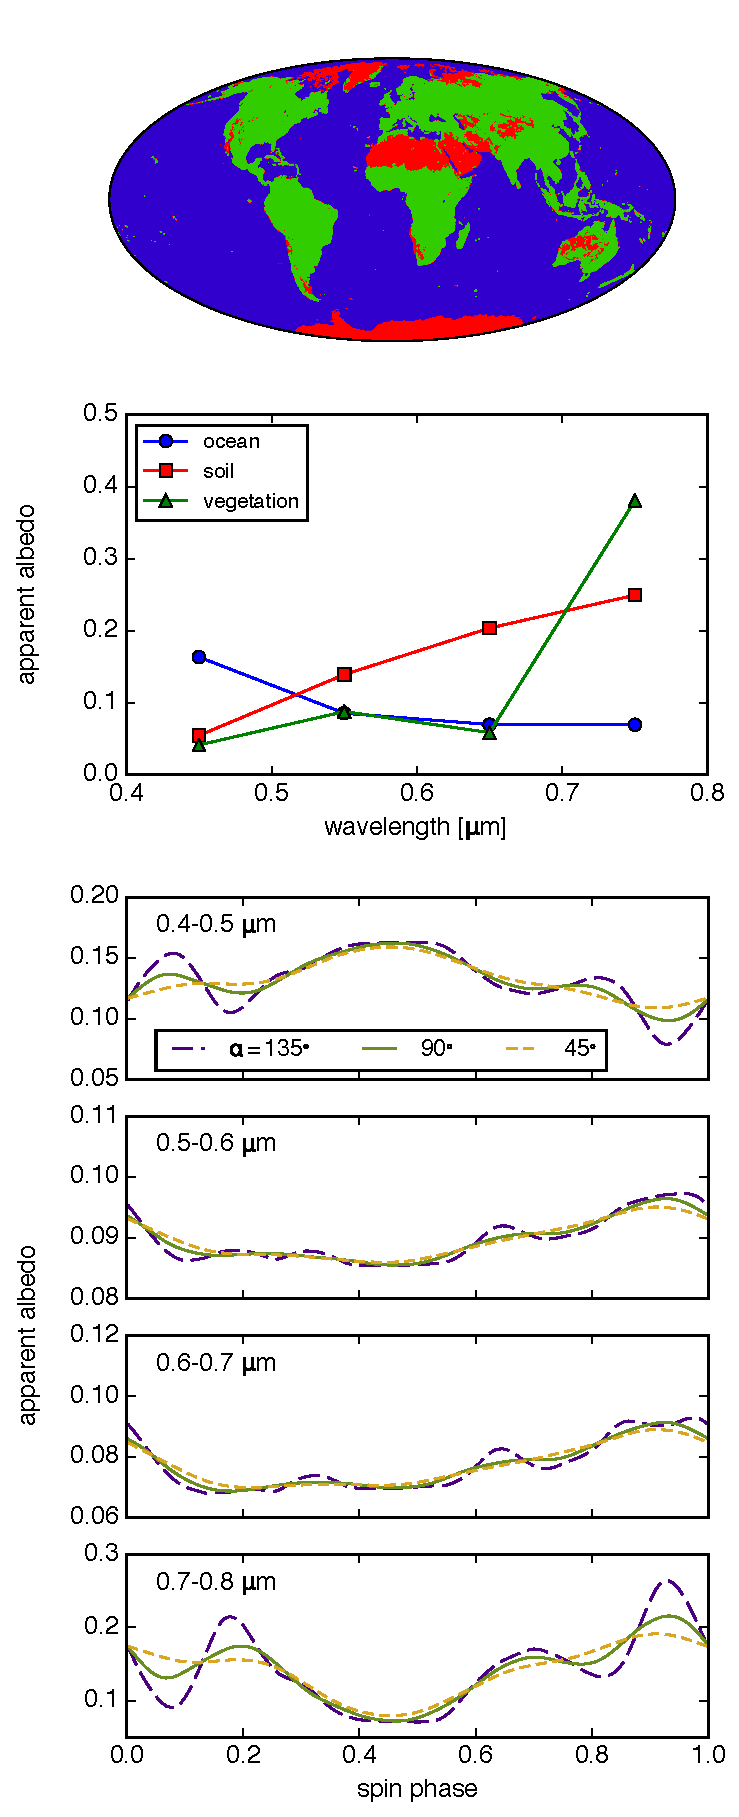
\includegraphics[width=\hsize]{mockdata.pdf}
%    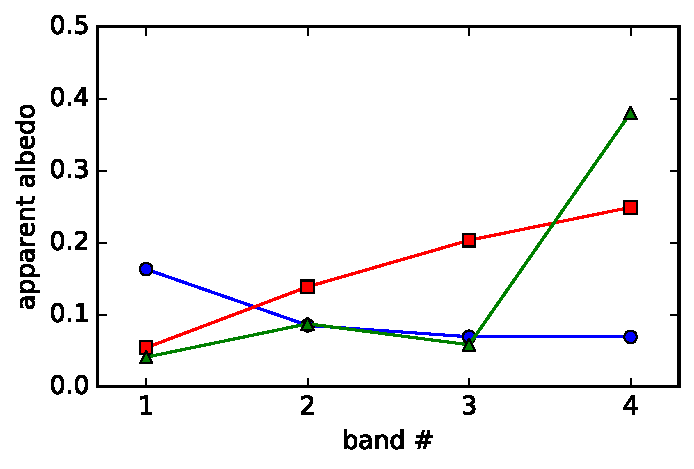
\includegraphics[width=\hsize]{mockdata_3types_albd.pdf}
%	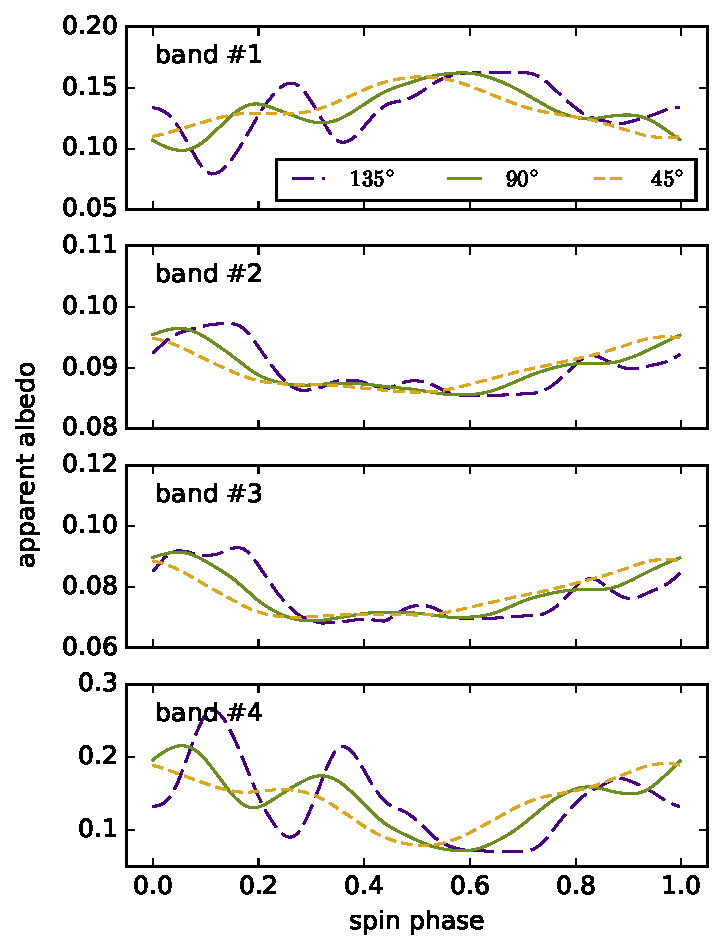
\includegraphics[width=\hsize]{mockdata_3types_t360_lc.pdf}
    \end{center}
    \caption{Our mock data based on IGBP classification map of the Earth. Top panel: distribution of 3 surface types (ocean: blue, soil: red, vegetation: green). Middle panel: assumed albedo spectra with matching colors. Bottom 4 panels: rotational light curves in 4 photometric band with varying phase angle, $\alpha = 135^{\circ }$ (purple, dot-dashed), $90^{\circ }$ (olive, solid), and $45^{\circ }$ (gold, dashed). }
\label{fig:mockdata}
\end{figure}
%%%%%%%%%%%%%%%%%%%%%%%%%%%%%%%%%%%


%%%%%%%%%%%%%%%%%%%%%%%%%%%%%%%%%%%%%%%%%%%%%%%%%%%%%%%%%%%%%%%%%%%
\section{Preparing Mock Datasets}
\label{s:mockdata}
%%%%%%%%%%%%%%%%%%%%%%%%%%%%%%%%%%%%%%%%%%%%%%%%%%%%%%%%%%%%%%%%%%%

The aim of this paper is to present how to constrain the albedo spectra of representative surface types from multi-band light curves. 
In order to facilitate the discussions about the procedures in the following sections, in this section we shall introduce a dataset to be used for demonstrations. 

We consider diurnal light curves of a toy model of the atmosphere-less Earth, in 4 photometric bands. 
We use a simplified surface map as shown in the upper left panel of Figure \ref{fig:mockdata}. 
This map is based on the land classification by the International Geosphere-Biosphere Programme (IGBP)\footnote{\url{https://climatedataguide.ucar.edu/climate-data/ceres-igbp-land-classification}}. 
Although the original classification assumes 16 land surface types plus ocean, in this paper we assume 3 surface types for simplicity regarding ``Open Shrubs'', ``Urban'', ``Snow/Ice'', and ``Barren/Desert'' as ``soil'' (red in the upper left panel of Figure \ref{fig:mockdata}) and other land surface types as ``vegetation'' (green), while keeping the ``ocean'' regions. 


The assumed albedo spectra of these surface types in 4 photometric bands are shown in the upper right panel of Figure \ref{fig:mockdata}. 
These 4 photometric bands actually correspond to the 0.4-0.5 $\mu $m, 0.5-0.6 $\mu $m, 0.6-0.7 $\mu $m, and 0.7-0.8 $\mu $m, respectively, but they will be simply called by the band indices unless otherwise noted . 
The albedo spectrum for ocean is based on \citet{Mclinden1997}, 
and the data for soil and vegetation are taken from ASTER spectral library\footnote{\url{https://speclib.jpl.nasa.gov/}. 
Specifically, we adopt  ``Brown to dark brown sand'' for ``soil'', and ``Grass'' for the ``vegetation''}. 
The scattering phase function by the surface is assumed to obey the Lambert law, i.e., the radiance is (incident flux)$\times $(albedo)/$\pi$, independent of the direction of the scattering. 

The light curves are synthesized given the relative potisions of the star, planet, and observer.  
For the sake of simplicity, we consider a planet with zero obliquity in an edge-on orbit, and change the phase angle (the planet-centric angle between the star and the observer) denoted by $\alpha $. 
However, the following discussion does not depend on these assumptions. 

The bottom panels of Figure \ref{fig:mockdata} display the examples of diurnal light curves in 4 photometric bands, represented in terms of {\it apparent albedo}. 
Apparent albedo is the planetary intensity normalized by that of a loss-less Lambert sphere with the same radius and at the same phase \citep{Qiu2003, Seager2010}; in this paper we will use apparent albedo unless otherwise noted. 
The apparent albedo is straightforwardly obtained from the observed planetary intensity, if and only if the planetary radius and the observational geometry are completely known: latitude/longitude of the sub-stellar/sub-observer points, and the distance between the star and the planet. 
\memoYF{Later in the paper, mention that the uncertainty in radius estimation severely affects the constraints. }
%(We will discuss the effect of this assumptions later in Section ??.)

The problem throughout this paper is, from this kind of multi-band diurnal light curves, how and how well we can retrieve the albedo spectra of different surface types as well as the longitudinal distribution of these surface types. 


%%%%%%%%%%%%%%%%%%%%%%%%%%%%%%%%%%%%%%%%%%%%%%%%%%%%%%%%%%%%%%%%%%%
\section{Inverse problem}
\label{s:frame}
%%%%%%%%%%%%%%%%%%%%%%%%%%%%%%%%%%%%%%%%%%%%%%%%%%%%%%%%%%%%%%%%%%%

In this section, we discuss the general framework to analyze the diurnal light curves, and present some demonstrations using the mock data created in the previous section. 
Sections \ref{ss:model} and \ref{ss:PCplane} are essentially the recapitulation of the previous papers, in particular \citet{Cowan2013} \citep[but see also][]{Cowan2009,Cowan2011,Fujii2010,Fujii2011}.  
We, however, choose to include these discussions as a baseline to establish the later arguments. 
\memoYF{Too many overlaps??}

%%%%%%%%%%%%%%%%%%%%%%%%%%%%%%%%%%%%%%%%%%%%%%%%%%%%%%%%%%%%%%
\subsection{Algebraic Formulation}
\label{ss:model}
%%%%%%%%%%%%%%%%%%%%%%%%%%%%%%%%%%%%%%%%%%%%%%%%%%%%%%%%%%%%%%


%%%%%%%%%%%%%%%%%%%%%%%%%%%%%%%%%%%
\begin{table}[b]
\caption{Indexes}
\begin{center}
\begin{tabular}{lcc} \hline \hline
Name & Symbol & Maximum \\ \hline
Observation Time & $i$ & I \\
Band & $j$ & J  \\
Surface Type & $k$ & K  \\
Longitudinal Slice  & $l$ & L \\ \hline
\end{tabular}
\end{center}
\label{tab:index}
\end{table}%
%%%%%%%%%%%%%%%%%%%%%%%%%%%%%%%%%%%


On the assumption that the planetary surface is Lambertian scatterer everywhere, and that it is composed of a certain number $K$ of spectrally distinct surface types, the disk-integrated scattered light is a weighted summation of the reflectance spectra of different surface types. 
Using the local surface albedo $s_{\vec \Omega }$, the zenith angle of the insolation, $\theta _0$, and the zenith angle of the observer $\theta _1$ (both defined at each surface point),
the apparent albedo of the planet, $d_{ij}$ (``$d$'' for data) is written as follows \citep[see][]{Fujii2010}: 
%%%
\begin{eqnarray}
d_{i} (\lambda_j) &=& \displaystyle \frac{ \int_{{\rm IV}_i} s_{\vec \Omega }(\lambda_j) \cdot \cos \theta_0 ({\vec \Omega}) \cdot \cos \theta_1 ({\vec \Omega}) \cdot d\vec \Omega }{ \int_{{\rm IV}_i}  \cos \theta_0 ({\vec \Omega}) \cdot \cos \theta_1 ({\vec \Omega}) \cdot d\vec \Omega } \\
&=& \sum _{k} s_k (\lambda_j) \; \displaystyle \frac{ \int_{{\rm IV}_{i}} f_k (\vec \Omega ) \cos \theta_0 ({\vec \Omega}) \cdot \cos \theta_1 ({\vec \Omega}) \cdot d\vec \Omega }{ \int_{{\rm IV}_i}  \cos \theta_0 ({\vec \Omega}) \cdot \cos \theta_1 ({\vec \Omega}) \cdot d\vec \Omega } \notag \\
&=& \sum _{i,k} \fast_{ik} \, s_{kj} \label{eq:tilde_d_f_ast_s}
\end{eqnarray}
%%%
where the surface spectra are:
%%%
\begin{equation}
s _{kj} \equiv  s_k (\lambda _j)
\end{equation}
%%%
and the apparent cover fractions are:
%%%
\begin{equation}
\tilde f_{ik} \equiv  \frac{ \int_{{\rm IV}_{i}} f_k (\vec \Omega ) \cos \theta_0 ({\vec \Omega}) \cdot \cos \theta_1 ({\vec \Omega}) \cdot d\vec \Omega }{ \int_{{\rm IV}_i}  \cos \theta_0 ({\vec \Omega}) \cdot \cos \theta_1 ({\vec \Omega}) \cdot d\vec \Omega }
\end{equation}
%%%
and $i$, $j$, and $k$ are indices for the observation epochs, bands, and the surface types, respectively, ${\rm IV }_i$ denotes the illuminated and visible area over the planetary surface at $i$-th observation, and $f (\vec \Omega )$ is the area fraction of $k$-th surface type in $d\vec \Omega$. 
In the last expression, $\fast_{ik}$ represents the apparent covering fraction of the $k$-th surface type at $i$-th observational epoch, and 
$s_{kj}$ is the reflectance spectra of $k$-th surface type at $j$-th band. 
The maximum number of $i$, $j$ and $k$ will be denoted by $I$, $J$, and $K$, below, as summarized in Table \ref{tab:index}. 

By definition, the area fraction, $\fast $, should not be negative and sum up to unity, and reflectance spectra, $s$, should be between 0 and 1. Therefore,
%%%
\begin{subnumcases}
{}
0 \leq \fast_{lk} \;\;\; & \mbox{for any $l$, $k$} \label{eq:tilde_f_range} \\
\sum_k \fast_{lk} = 1 & \mbox{for any $l$} \label{eq:tilde_f_sum} \\
0 \leq s_{kj} \leq 1 \;\;\; & \mbox{for any $k$, $j$} \label{eq:tilde_s_range} 
\end{subnumcases}
%%%


%%%
%\begin{eqnarray}
%\begin{cases}
%\;\; 0 \leq s_{kj} \leq 1 \;\;\; & \mbox{for any $k$, $j$} \\
%\;\; 0 \leq \fast_{lk} \leq 1 \;\;\; & \mbox{for any $l$, $k$} \label{eq:cond_f_ast}\\
%\;\; \sum_k \fast_{lk} = 1 & \mbox{for any $l$} 
%\end{cases}
%\end{eqnarray}
%%%

%\subsection{Estimating the Composition\\of Longitudinal Slices}

The time variability of the apparent covering fraction $\fast $ due to the planet's rotation is related to the surface inhomogeneity along the equator. Approximately, $\fast _{ik}$ may be written as the weighted summation of the area fraction of $k$-th surface type in each of (the finite number $L$ of) longitudinal slices, i.e.,
%%%
\begin{eqnarray}
\fast _{ik} &=& \frac{ \int_{{\rm IV}_{i}} f_k (\vec \Omega ) \cos \theta_0 ({\vec \Omega}) \cdot \cos \theta_1 ({\vec \Omega}) \cdot d\vec \Omega }{ \int_{{\rm IV}_i}  \cos \theta_0 ({\vec \Omega}) \cdot \cos \theta_1 ({\vec \Omega}) \cdot d\vec \Omega }  \\
&=& \sum_l \frac{ \int_{{\rm IV}_{il}}  f_k (\vec \Omega ) W (\vec \Omega  ) \cdot d\vec \Omega }{ \int_{{\rm IV}}  W (\vec \Omega ) \cdot d\vec \Omega } \\
&\approx & \sum_l f_{lk} \frac{ \int_{{\rm IV}_{il}} W (\vec \Omega ) \cdot d\vec \Omega }{ \int_{{\rm IV}}  W (\vec \Omega ) \cdot d\vec \Omega } \label{eq:discretize}\\
&\equiv & \sum_l  W_{il} f_{lk} \label{eq:Wf}, 
\end{eqnarray}
%%%
where $l$ is the index for longitudinal slices, $f_{lk}$ is the area fraction of the $k$-th surface type in the $l$-th longitudinal slice. 
Strictly speaking, the approximation is valid only when $f_k(\vec \Omega)$ does not change or changes little across the $l$-th slice for all $k$ and $l$. 
\memoYF{Comment from Nick: is this approximation exact in the zero obliquity, edge-on limit?}
In the last equation, $W_{il}$ is the weight function for $i$-th epoch and $l$-th longitudinal slice which depends only on the observational geometry. 
As a result,
%%%
\begin{equation}
d_{ij} = \sum _{l,k} W_{il} \, f_{lk} \, s_{kj} \label{eq:d_f_s}
\end{equation}
%%%
where $f_{lk}$ is the average area fraction of $k$-th surface type at $l$-th longitudinal slice, Again, the area fractions at longitudinal slices, $f_{lk}$, cannot be negative and should sum up to unity. Thus, a set of condition similar to Equations (\ref{eq:tilde_s_range})-(\ref{eq:tilde_f_sum}) are imposed:
%%%
\begin{subnumcases}
{}
0 \leq f_{lk} \;\;\; & \mbox{for any $l$, $k$} \label{eq:f_range} \\
\sum_k f_{lk} = 1 & \mbox{for any $l$} \label{eq:f_sum} \\
0 \leq s_{kj} \leq 1 \;\;\; & \mbox{for any $k$, $j$} \label{eq:s_range}
\end{subnumcases}
%%%
Now, the relevant problem is, given $d$, estimate $\{f, s\}$ subject to the constraints of Equations (\ref{eq:s_range})-(\ref{eq:f_sum})---this is where \citet{Cowan2013} stood. 


%\citet{Cowan2013} proposed the specific procedure to find the solution for $\{f, s\}$. 
%Namely, 
%(1) perform PCA on the data to reduce the dimensionality as needed, 
%(2) perform simplex shrink-wrapping analysis to find the first guess for $s$, 
%and 
%(3) find the maximum posterior values for $\{f, s\}$ using MCMC algorithm  and setting the first guess for $s$ as the initial condition. 
%(The initial value for $f$ is fixed at 1/(\# of surface types).)

%\newpage


%%%%%%%%%%%%%%%%%%%%%%%%%%%%%%%%%%%
\begin{figure}[b!]
    \begin{center}
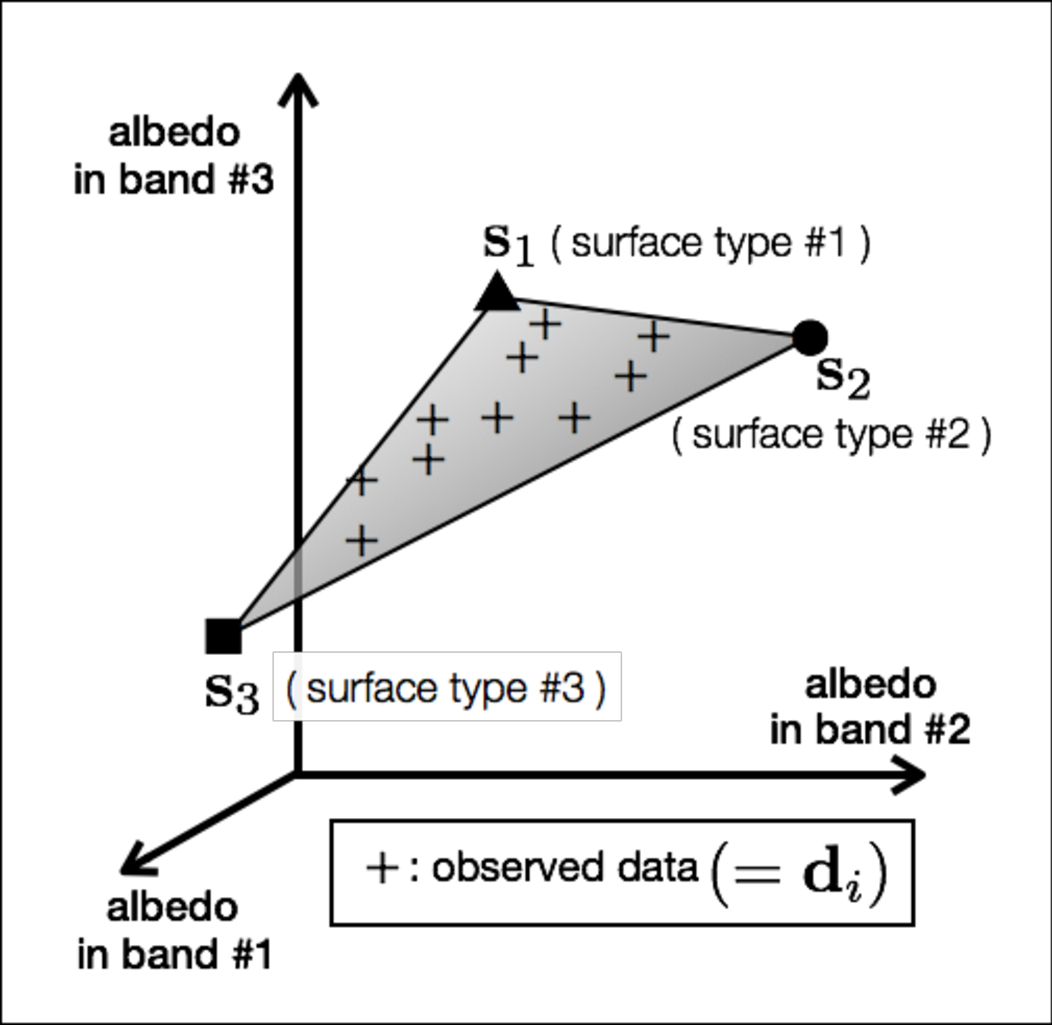
\includegraphics[width=\hsize]{schematics.pdf}
    \end{center}
    \caption{Schematic figure to illustrate the relation between $\{{\bf s}_k\} $ and $\{{\bf d}_i\} $ (see text). }
\label{fig:schematic}
\end{figure}
%%%%%%%%%%%%%%%%%%%%%%%%%%%%%%%%%%%


%%%%%%%%%%%%%%%%%%%%%%%%%%%%%%%%%%%%%%%%%%%%%%%%%%%%%%%%%%%%%%
\subsection{Graphical Conception on \\Principal Component (Hyper-)Plane}
\label{ss:PCplane}
%%%%%%%%%%%%%%%%%%%%%%%%%%%%%%%%%%%%%%%%%%%%%%%%%%%%%%%%%%%%%%

%A question is whether the above formulation leads us to a unique solution of either $\{ {\bf \fast},\,{\bf s} \}$ or $\{ {\bf f},\,{\bf s}\}$, given the data matrix, ${\bf d}$. 

Equation (\ref{eq:tilde_d_f_ast_s}) coupled with the conditions (\ref{eq:tilde_f_range}) and (\ref{eq:tilde_f_sum}) indicates the geometrical relationship among ${\bf d}$, ${\bf \fast }$, and ${\bf s}$ in the $J$-th dimensional space, where $\{{\bf d}_i\}$ correspond to the points that are located on the (hyper-)plane defined by $K$ ($<J$) number of points, $\{{\bf s}_k\} $, and are enclosed by $\{{\bf s}_k \}$. \memoYF{How is it called in one word in mathematics?}
Figure \ref{fig:schematic} graphically shows this relations in the case of $J=3$ and $K=3$. 
Note that the dimension of this (hyper-)plane is $K-1$; In other words, the number of spectrally distinct major surface types ($=K$) is the number of dominant principal components (PCs) plus 1 in theory \citep{Cowan2011}. 
%We show this graphically in Figure \ref{fig:trajectory}, using the mock datasets shown in Section \ref{s:mockdata}. 

This (hyper-)plane can be identified through Principal Component Analysis (PCA) \citep{Cowan2009,Cowan2011}, as PCA extracts the major axes along which the scatter among the data points are significant. 
% used Principal Component Analysis (PCA) to 
% The original data, however, have 4 photometric bands (i.e., $J=4$), and $J$-the dimensional space is inconvenient for visualization. 
We thus start by performing principal component analysis (PCA). 
From the mock light curves prepared in Section \ref{s:mockdata}), we extract two dominant PCs through PCA (other components are found to have virtually zero contribution). 
The PCs extracted from the light curves at $\alpha = 90^{\circ }$ (olive lines in Figure \ref{fig:mockdata}) are presented in Figure \ref{fig:PCs}. 
In the following, we adopt these two PCs as the axes of the PC plane. \memoYF{Comment from Nick: This is true by definition?}
Although the PCs from other light curves with different phase angles are not necessarily same as the one shown in Figure \ref{fig:PCs}, the PC plane itself should be the same plane, because we assume the same 3 surface types (under the noiseless condition). Thus it is ok to use these PCs to discuss other light curves as well. 

Figure \ref{fig:trajectory} shows the trajectories of the mock light curves with varying phase angle on the plane defined by PC 1 and PC 2. 
The excursion of the trajectory is larger for the light curve at a larger phase angle, i.e., at crescent phase, and shrinks as the phase angle decreases because a larger surface area is averaged together.  
The points in the figure indicate the input albedo spectra of the three surface types. 
As described above, the trajectories are always inside the triangle defined by these points. 
%Because the apparent albedo at any time of the observations is a linear combination of input surface colors (Equation \ref{eq:tilde_d_f_ast_s}) under the conditions (\ref{eq:tilde_f_range}) and (\ref{eq:tilde_f_sum}), the trajectories should always be inside the triangle defined by these points.  



 
%%%%%%%%%%%%%%%%%%%%%%%%%%%%%%%%%%%
%\begin{figure}[tbh!]
%    \begin{center}
%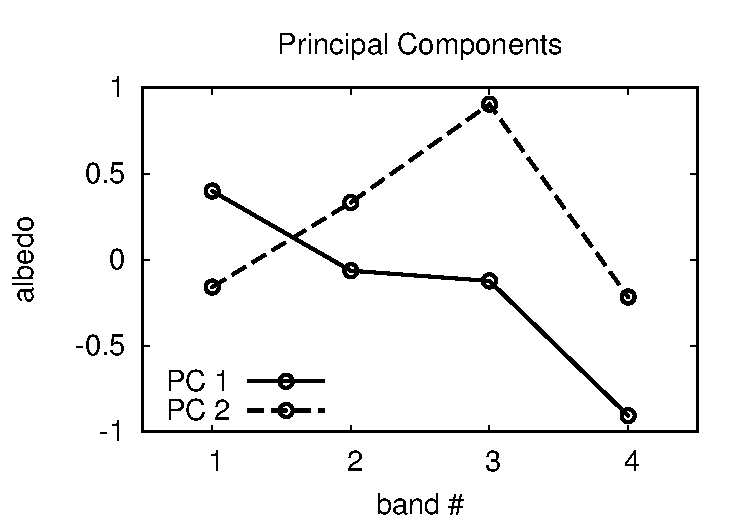
\includegraphics[width=\hsize]{PCA_V_jn.pdf}
%    \end{center}
%    \caption{Principal components of the light curves shown in the bottom of Figure \ref{fig:mockdata}. }
%\label{fig:PCs}
%\end{figure}
%%%%%%%%%%%%%%%%%%%%%%%%%%%%%%%%%%%

%%%%%%%%%%%%%%%%%%%%%%%%%%%%%%%%%%%
\begin{figure}[t]
    \begin{center}
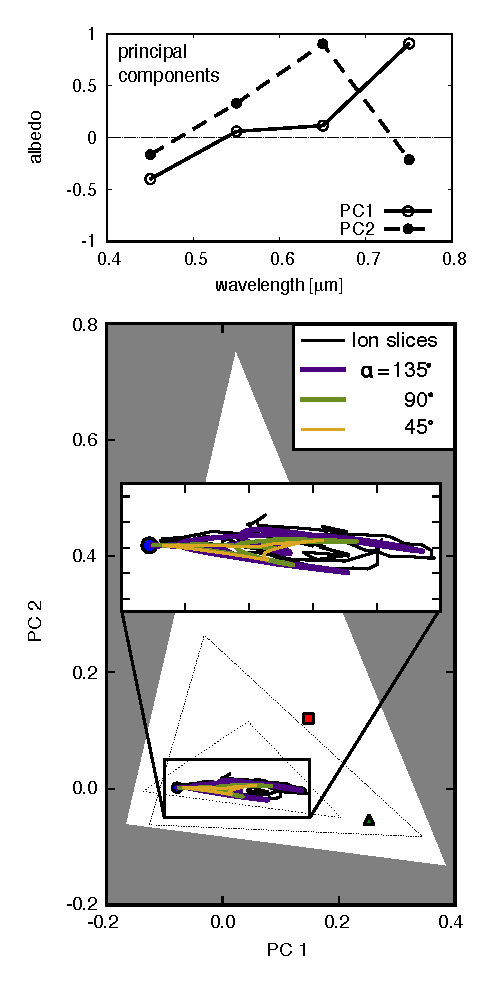
\includegraphics[width=\hsize]{mockdata_PCplane.pdf}
    \end{center}
    \caption{Upper panel: principal components (PCs) of the light curves at $\alpha = 90^{\circ }$ shown in olive lines in Figure \ref{fig:mockdata}. Lower panel: trajectories of the 4-band light curves on the PC plane set by 2 PCs shown in the upper panel, in the case of $\alpha = 135^{\circ }$ (indigo thick line), $\alpha = 90^{\circ }$ (olive line), and $\alpha = 45^{\circ }$ (gold thin line). Points indicate the input albedo spectra of ocean (blue circle), soil (red square), and vegetation (green triangle) on the PC plane. Points in the gray region violate the condition (\ref{eq:tilde_s_range}); specifically, the left, right, and bottom boundaries are set by $s_{k,4}> 0$, $s_{k,1}> 0$, and $s_{k,3}> 0$, respectively. 
Dotted lines are random triangle that could be solutions (see text). \memoYF{I have to redo the first panel!!}}
    \label{fig:trajectory}
\end{figure}
%%%%%%%%%%%%%%%%%%%%%%%%%%%%%%%%%%%

%%%%%%%%%%%%%%%%%%%%%%%%%%%%%%%%%%%%%%%%%%%%%%%%%%%%%%%%%%%%%%
\subsection{Formal Degeneracy}
\label{ss:degeneracy}
%%%%%%%%%%%%%%%%%%%%%%%%%%%%%%%%%%%%%%%%%%%%%%%%%%%%%%%%%%%%%%

On the other hand, when it comes to the stage where we must estimate the surface spectra given the trajectory/-ies, {\it any} set of $\{ {\bf s}_k \}$ that enclose the data points $\{{\bf d}_i\}$ in the hyperplane can be a solution of Equation (\ref{eq:tilde_d_f_ast_s}) subject to the conditions (\ref{eq:tilde_f_range}) and (\ref{eq:tilde_f_sum}). 
Note that the associated matrix, $\fast _{ik}$, can always be found. 
Additional constraint comes from the condition (\ref{eq:tilde_s_range}). 
In Figure \ref{fig:trajectory} any points in the shadowed region are rejected based on this condition (the specific inequalities corresponding to the border lines are noted in the figure caption. ). 
While this limits the region where $\{ {\bf s}_k \}$ can exist,   
this is in general not sufficient to result in a unique solution. 
In Figure \ref{fig:trajectory} we show two random triangles that enclose the trajectory; these triangles satisfy the conditions, so do many others. 
One can have spectrally interesting surface spectra and boring geography (small longitudinal variation in area fractions) {\it or} one can have boring surface spectra (closer to flat) and interesting geography. \memoYF{Need to reconsider this phrasing. }
Therefore, predicting ${\bf \fast }$ and ${\bf s}$ from ${\bf d}$ is clearly a ill-posed problem. 





A formally equivalent degeneracy is found in Equation (\ref{eq:d_f_s}) coupled with the conditions (\ref{eq:f_range})-(\ref{eq:s_range}). 
Essentially, the term $\sum _k f_{lk} s_{kj}$ represents the average albedo spectra of $l$-th slice and $W_{il}$ is the matrix that convolve them into the light curves. 
But again, we can have different sets of $\{ {\bf s}_k \}$ that enclose the averaged albedo spectra of longitudinal slices {\it and} are located in the range of condition (\ref{eq:s_range}), any of which can make up the given averaged albedo spectra with the associated $f_{lk}$. 
For disk-integrated light curves, the color excursions are more muted than the intrinsic longitudinal map, so the degeneracy becomes severer. 

%%%%%%%%%%%%%%%%%%%%%%%%%%%%%%%%%%%%%%%%%%%%%%%%%%%%%%%%%%%%%%
\subsection{Constraining the Surface Types}
\label{ss:constraining}
%%%%%%%%%%%%%%%%%%%%%%%%%%%%%%%%%%%%%%%%%%%%%%%%%%%%%%%%%%%%%%


%%%%%%%%%%%%%%%%%%%%%%%%%%%%%%%%%%%
\begin{figure*}[tbh!]
   \begin{minipage}{0.33\hsize}
    \begin{center}
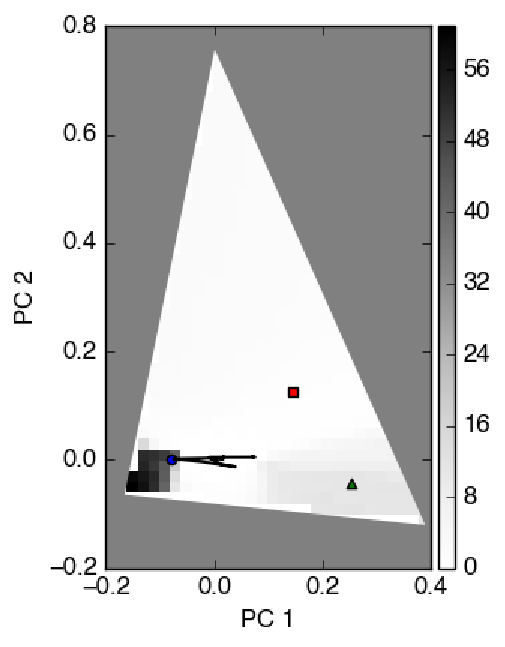
\includegraphics[width=\hsize]{mockdata_90deg_3types_t12_lc_noreg.pdf}
    \end{center}
     \end{minipage}   
    \begin{minipage}{0.33\hsize}
    \begin{center}
%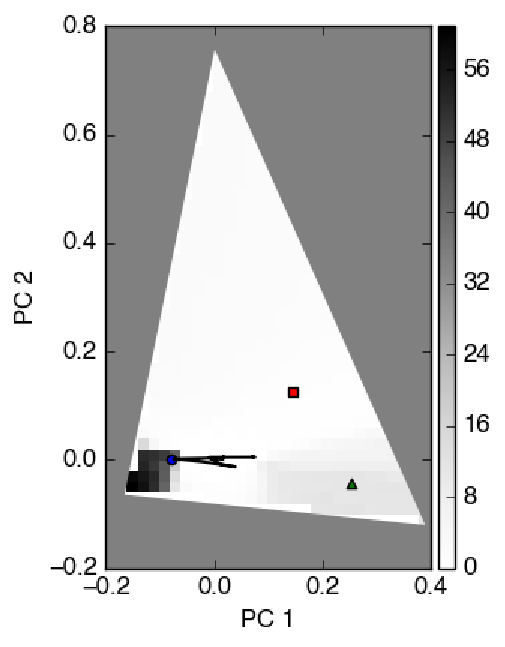
\includegraphics[width=\hsize]{mockdata_90deg_3types_t12_lc_noreg.pdf}
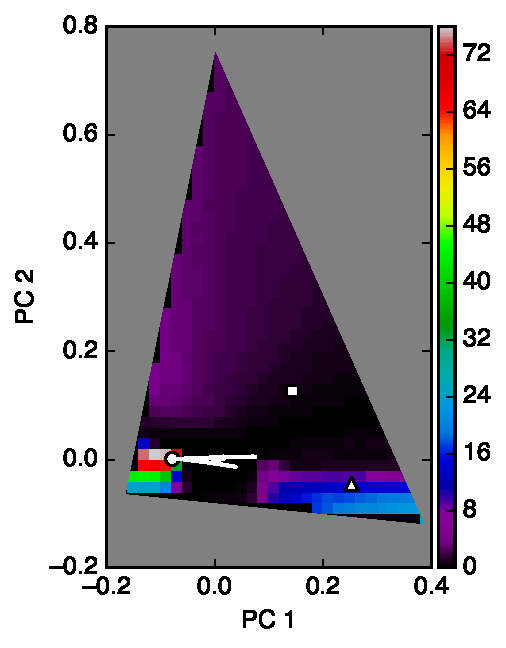
\includegraphics[width=\hsize]{mockdata_90deg_3types_t12_lc_reg_l30deg.pdf}
    \end{center}
     \end{minipage}
   \begin{minipage}{0.33\hsize}
    \begin{center}
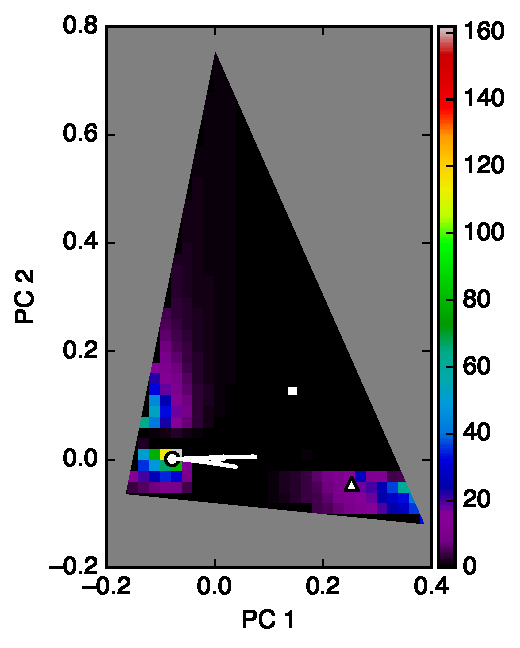
\includegraphics[width=\hsize]{mockdata_90deg_3types_t12_lc_reg_l40deg.pdf}
    \end{center}
     \end{minipage}
    \caption{Left: Probability of surface albedo spectra estimated from colors of longitudinal slices, without regularization term (``flat'' prior?). Middle: on the assumption of gaussian process with correlation length $30^{\circ }$. Right panel: correlation length $40^{\circ }$. }
\label{fig:noreg}
\end{figure*}
%%%%%%%%%%%%%%%%%%%%%%%%%%%%%%%%%%%


Given that any combinations that enclose the trajectory/-ies can be a solution, the choice of the solution critically depends on the prior probability distribution. 
% Thus, we need to be careful about the implicit assumptions that are made  
With no assumptions or information on the spectral albedo of the surface types or geography, it may be reasonable to assume that any points in the PC plane except for the inhibited regions are equally likely to correspond to a surface type. 
While such an assumption does not seem to work at all to choose the surface types, it does put some constrains. 
This is because of the relative configuration of the trajectory and the permitted region. 
For example, in Figure \ref{fig:trajectory}, in order to enclose the trajectory with three surface types within the permitted region, we must have at least one point near the bottom left corner of the permitted region (white triangle); this is consistent with the fact that one of the input albedo spectra (ocean) resides there. 

In order to see this more quantitatively, we make a grid on the PC plane  with an interval of 0.2 and consider all combinations of three grid points. 
Then, we assumed that all of the combinations that enclose the trajectory (in the case of $\alpha =90^{\circ }$) are equally likely to be a solution, and found the marginalized probability of having a surface type at each location of the PC plane, as shown in Figure \ref{fig:noreg}. 
%
As expected, we find a relatively definite peak near the point of ocean. 
On the other hand, the peak that corresponds to soil is a blur, and it is almost not constrained. 
The vegetation in the bottom right corner is moderately constrained. 



%%%%%%%%%%%%%%%%%%%%%%%%%%%%%%%%%%%%%%%%%%%%%%%%%%%%%%%%%%%%%%
\subsection{Additional Constraints}
\label{ss:regularization}
%%%%%%%%%%%%%%%%%%%%%%%%%%%%%%%%%%%%%%%%%%%%%%%%%%%%%%%%%%%%%%


%%%%%%%%%%%%%%%%%%%%%%%%%%%%%%%%%%%%%%%%%%%%%%%%%%%%%%%%%%%%%%
%\section{Constraining the Surface Types}
%\label{ss:constraining}
%%%%%%%%%%%%%%%%%%%%%%%%%%%%%%%%%%%%%%%%%%%%%%%%%%%%%%%%%%%%%%


%%%%%%%%%%%%%%%%%%%%%%%%%%%%%%%%%%%%%%%%%%%%%%%%%%%%%%%%%%%%%%
%\subsection{Prior: Gaussian Processes}
%\label{ss:gp}
%%%%%%%%%%%%%%%%%%%%%%%%%%%%%%%%%%%%%%%%%%%%%%%%%%%%%%%%%%%%%%

\memoYF{This is just a quick draft and will need to be updated significantly.}

A more constraining condition we might impose is the correlation length of the light curves. 
This accounts to assuming a longitudinal correlation length in the planet's geography. 

%%%
\begin{eqnarray}
&&Posterior 
\\ &&= \prod\limits_{i,j}\left[  \frac{1}{\sqrt{2\pi }\sigma_{ij}} \exp \left\{ - \frac{(d_{ij} - \sum _{lk} W_{il} f_{lk} s_{kj})^2}{2 \sigma _{ij}^2} \right\} \right] \notag \\
&& \;\;\;\;\;\;\;\;\;\; \times \; \mathcal{P} (\{f_{lk}\}) \cdot \mathcal{P}(\{s_{kj}\}) 
\end{eqnarray}
%%%
where $\mathcal{P} (X) $ is a prior for $X$. 

The assumption of smooth time variation of covering area fraction may be imposed using the concept of Gaussian Process \citep{Rasmussen2005}. 
We assume that the variation of the covering fraction follows Gaussian Process, which means the any finite number of the covering fractions have a joint Gaussian distribution. 
Such assumption can be represented by the prior of 
%%%
\begin{equation}
\mathcal{P}_{\fast} = \frac{1}{\sqrt{ 2 \pi }^{L(K-1)} \sqrt{| \tilde \Sigma |} } \exp( - \fast^{T} \tilde \Sigma ^{-1} \fast ) 
\end{equation}
%%%
or
%%%
\begin{equation}
\mathcal{P}_f = \frac{1}{\sqrt{ 2 \pi }^{L(K-1)} \sqrt{| \Sigma  |}} \exp( - f^{T} \Sigma ^{-1} f ) 
\end{equation}
%%%
where $\Sigma $ is the kernel representing the property of the gaussian processes assumed for $f$.
In this paper, we assume squared exponential covariance function, i.e., 
%%%
\begin{equation}
\tilde \Sigma _{ii'} = \lambda \exp \left( - \frac{|t_i- t_i'|^2}{2 (\Delta t_0) ^2} \right)
\end{equation}
%%%
where $t_i$ is the time of $i$-th observation and $(\Delta t_0)$ is characteristic time scale over which $\fast $ is supposedly correlated, or 
%%%
\begin{equation}
\Sigma _{ll'} = \lambda \exp \left( - \frac{|\phi_l- \phi_{l'}|^2}{2 \phi_0^2} \right)
\end{equation}
%%%
where $\phi_l$ is the longitude of $l$-th slice, and $\phi_0$ is the characteristic longitudes over which $f$ is correlated.  



%%%%%%%%%%%%%%%%%%%%%%%%%%%%%%%%%%%
\begin{figure}[tbh!]
    \begin{center}
%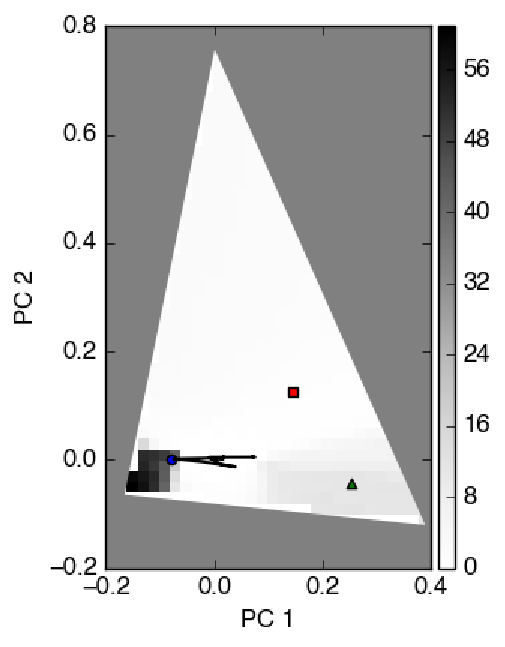
\includegraphics[width=\hsize]{mockdata_90deg_3types_t12_lc_noreg.pdf}
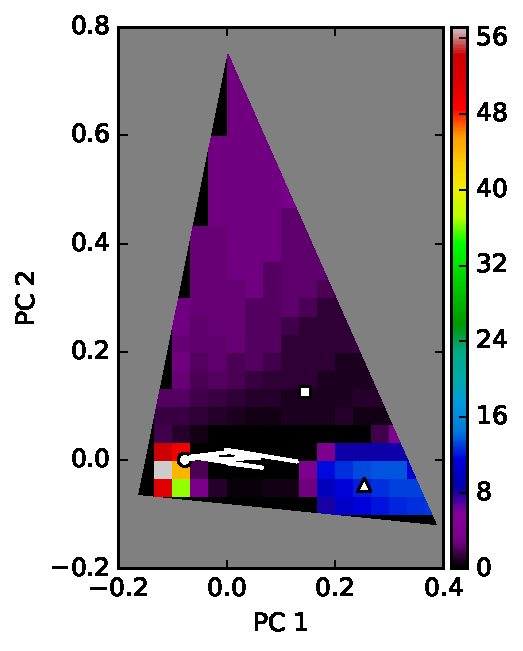
\includegraphics[width=\hsize]{IGBP_lon_noreg.pdf}
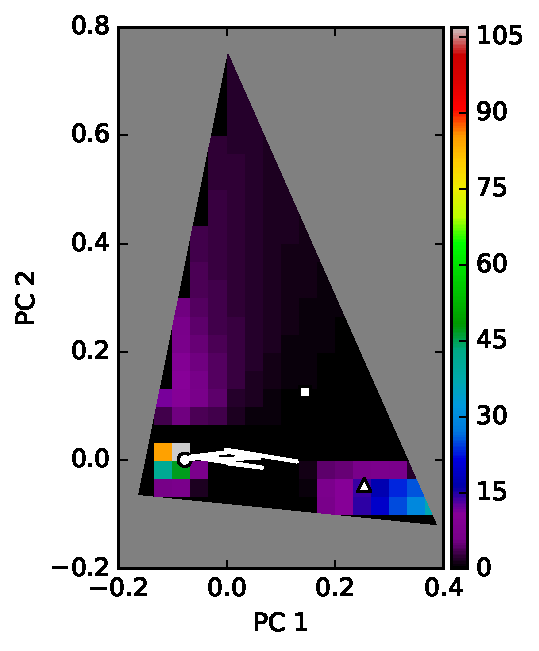
\includegraphics[width=\hsize]{IGBP_lon_reg_l30deg.pdf}
    \end{center}
    \caption{Probability of surface albedo spectra estimated from colors of longitudinal slices, without (upper) and with (lower) regularization term. The regularization term for the lower panel assumes correlation length $30^{\circ }$. }
\label{fig:noreg}
\end{figure}
%%%%%%%%%%%%%%%%%%%%%%%%%%%%%%%%%%%


\bibliography{ref}


\end{document}






%%%%%%%%%%%%%%%%%%%%%%%%%%%%%%%%%%%%%%%%%%%%%%%%%%%%%%%%%%%%%%
\subsection{Fit data with $\fast $ or with $f$ ?}
\label{ss:degeneracy}
%%%%%%%%%%%%%%%%%%%%%%%%%%%%%%%%%%%%%%%%%%%%%%%%%%%%%%%%%%%%%%

\memoYF{I am not 100\% sure if the following statement is right. Need to check. The argument below probably makes sense for the noiseless case. What if the data are noisy?}
 
We argue that estimating $\{ f, s \}$ is no superior to estimating $\{ \fast, s \}$. 
%
One reason comes from the approximation adopted in equation (\ref{eq:discretize}) is valid only when $f_k (\vec \Omega)$ does not change significantly in the $l$-th slice. 
Otherwise, fitting data with $f$ by equation (\ref{eq:Wf}) produces some errors by design. 

%Suppose the above approximation is justified. 
In essence, $\fast_{ik}$ and $f_{lk}$ contains the same information, where they are related through a fixed $W_{il}$ (eq. \ref{eq:Wf}). 
%
If $L=I$, in general there is a one-to-one relationship between $\fast_{ik}$ and $f_{lk}$ through $W_{il}$ as far as ${\rm rank}(W)=L(=I)$. 
In this case, clearly, equations (\ref{eq:cond_f_ast}) and (\ref{eq:cond_f}) are equivalent, given $W_{il}>0$ (for any $i$ and $j$) and $\sum _l W_{il} = 1$. 
%
If $L<I$, the matrix $W$ works as a low-pass filter \citep{Cowan2013}. 
In this case, the inverse problem described by equation (\ref{eq:Wf}), $\fast=Wf$, is an overdetermined system, and one must to find the solution for $f$ by some means (e.g. the least squares method), and the resultant $f$ may not automatically satisfy the condition listed by equation (\ref{eq:cond_f}). 

However, this is because of the design of the problem and the assumed lowered resolution. 

Therefore, although either $\{ \fast, s \}$ or $\{ f, s \}$ could be fitting parameters to the data, the estimation for $s$ should not be affected by this conversion in fitting parameters. 
In that sense, $\{ f, s \}$ is not likely to return a better solution than $\{ \fast, s \}$ does. 
Rather, it could return less reasonable results because of the approximation adopted in equation (\ref{eq:discretize}). 

\newpage

%%%%%%%%%%%%%%%%%%%%%%%%%%%%%%%%%%%%%%%%%%%%%%%%%%%%%%%%%%%%%%
\subsection{Degeneracy}
\label{ss:degeneracy}
%%%%%%%%%%%%%%%%%%%%%%%%%%%%%%%%%%%%%%%%%%%%%%%%%%%%%%%%%%%%%%

\memoYF{The degeneracy in solving $\{ \fast ,\,s\} $ is already indicated in \citet{Cowan2013}, but might be worth clarifying here again. }


One could try to find the solutions for $\{ \fast, s \}$ given $d$ using equation (\ref{eq:d_f_ast_s}), or the solutions for  $\{ f, s \}$ using equation (\ref{eq:d_f_s}), but we must keep in mind that 
these two formulations both embrace intrinsic degeneracies in the solutions if there is no other information about $\fast$ (or $f$) and $s$. 

%%%
%\begin{equation}
%d_{ij} = \sum _{i,k} f^{\ast }_{ik} \, s_{kj} \tag{\ref{eq:d_f_ast_s}}
%\end{equation}
%%%
%When one tries to find solutions for both $\fast$ and $s$ given $d$, the results are strongly degenerate if there are not other information about $\fast$ and $s$. 

Without any constraints on $\fast$ (or $f$) and $s$, it is trivial to notice the degeneracy in the solutions. 
Using an arbitrary regular matrix $X$ with rank $K$, a particular set of solution $\{ \fast ,\,s\}$ implies another set of solution $\{ \fast X^{-1},\,Xs\}$. 

Now that they are subject to the constraints (equation (\ref{eq:cond_f_ast}) or (\ref{eq:cond_f})), the range of the acceptable solution is limited. Nevertheless, the constraints cannot be sufficient to narrow them to a unique set of solution. 
%
To see this, %let us consider equation (\ref{eq:d_f_ast_s}) for the moment.
imagine a $J$-dimensional space.
Suppose there are $K$ number of vertices in that space, $\vec x_1,\,\vec x_2,\,...,\,\vec x_K$, and that all of the coordinate of $\vec x_k$ in this $J$-dimensional space is between 0 and 1. 
Mathematically, any points (say, $\vec y_1$, $\vec y_2$, ..., $\vec y_I$) that are {\it enclosed} in the hyperplane defined by these vertices may be represented by $\vec y_i=\sum _k^K p_{ik} \vec x_k $ where $\sum _k^K p_{ik} = 1$ for any $i$. 
%In the matrix form, $Y_{ij} = P_{ik} X_{kj}$. 
This is essentially same as the situation described by equation (\ref{eq:d_f_ast_s}). 

In other words, any set of vertices in $J$-dimensional space that can enclose all of the observed data, $\vec d_i$ can be the solutions for equation (\ref{eq:d_f_ast_s}), as long as all of the element in $x_{kj}$ satisfy $0<x_{kj}<1$. 
The condition $0<x_{kj}<1$ generally constrains the outer boundary of the possible locations for the vertices. 
Therefore, the ``answer'' vertices allowed by the observations are somewhere outside the polygon that tightly encloses the observed data and inside the outer boundary defined by the condition $0<x_{kj}<1$ (see \S\ref{ss:shrinkwrap} below). 

Note that in an exceptional case where the apparent covering fractions of all of the surface type come close to unity to different epochs, the allowed region for the vertices would be narrow, i.e., better estimation can be expected. 


\newpage

%%%%%%%%%%%%%%%%%%%%%%%%%%%%%%%%%%%%%%%%%%%%%%%%%%%%%%%%%%%%%%
\subsection{Bayesian Formulation ?}
\label{ss:regularization}
%%%%%%%%%%%%%%%%%%%%%%%%%%%%%%%%%%%%%%%%%%%%%%%%%%%%%%%%%%%%%%

Assuming the observational noise is distributed as Gaussian, 
%%%
\begin{eqnarray}
&&Posterior 
\\ &&= \prod\limits_{i,j}\left[  \frac{1}{\sqrt{2\pi }\sigma_{ij}} \exp \left\{ - \frac{(d_{ij} - \sum _{lk} W_{il} f_{lk} s_{kj})^2}{2 \sigma _{ij}^2} \right\} \right] \notag \\
&& \;\;\;\;\;\;\;\;\;\; \times \; \mathcal{P} (\{f_{lk}\}) \cdot \mathcal{P}(\{s_{kj}\}) 
\end{eqnarray}
%%%
where $\mathcal{P} (X) $ is a prior for $X$. 

In order to take account of constraints (equation (\ref{eq:constraints})), we adopt the following transformation of variables: 
%%%
\begin{eqnarray}
\begin{cases}
t_{kj} = \displaystyle \ln \left[ \frac{ s_{kj} }{1 - s_{kj} } \right]  \;\;\; & \mbox{for any $k$, $j$} \\
g_{lk} = \displaystyle \ln \left[ \frac{ f_{lk} }{1 - \sum _{m=0}^{k} f_{lm} } \right] \;\;\; & \mbox{for $k=1, ..., K-1$} %, any $j$} 
\end{cases}
\end{eqnarray}
%%%
Note that there is a 1-to-1 correspondence between $t$ and $s$ or $g$ and $f$ where $s$. 

\newpage

%%%%%%%%%%%%%%%%%%%%%%%%%%%%%%%%%%%%%%%%%%%%%%%%%%%%%%%%%%%%%%
\subsection{Prior: Gaussian Processes}
\label{ss:gp}
%%%%%%%%%%%%%%%%%%%%%%%%%%%%%%%%%%%%%%%%%%%%%%%%%%%%%%%%%%%%%%

\memoYF{This is just a quick draft and will need to be updated significantly.}

As seen in Section \ref{ss:degeneracy}, the solution is highly degenerate, and in general we cannot reduce to a unique solution. 
Therefore, we may want to give a prior in estimating the area fractions. 
What kind of assumptions can we make?

In general, the large time/longitude variations in apparent area fractions corresponds to spectrally similar surface types, because such solution correspond to the proximity of the inner boundary in the $J$-dimensional space discussed above. 
On the contrary, spectrally well-separated surface types correspond to small time/longitude variations in the apparent area fractions. 
In the real world, we might expect that the latter is more likely, i.e., covering area fraction of any surface type would not change significantly along the longitude (or in time). 
This would be a reasonable assumption for the estimation of $\{s, \fast \}$, since the illuminated and visible area is usually broad and tend to change the averaged area fraction of each surface type only gently. 
Although there is no physical proof for this assumption...

The assumption of the smoothness of the time variation of covering area fraction may be imposed using the concept of Gaussian Process \citep{Rasmussen2005}. 
We assume that the variation of the covering fraction follows Gaussian Process, which means the any finite number of the covering fractions have a joint Gaussian distribution. 
Such assumption can be represented by the prior of 
%%%
\begin{equation}
\mathcal{P}_{\fast} = \frac{1}{\sqrt{ 2 \pi }^{L(K-1)} \sqrt{| \tilde \Sigma |} } \exp( - \fast^{T} \tilde \Sigma ^{-1} \fast ) 
\end{equation}
%%%
or
%%%
\begin{equation}
\mathcal{P}_f = \frac{1}{\sqrt{ 2 \pi }^{L(K-1)} \sqrt{| \Sigma  |}} \exp( - f^{T} \Sigma ^{-1} f ) 
\end{equation}
%%%
where $\Sigma $ is the kernel representing the property of the gaussian processes assumed for $f$.
In this paper, we assume squared exponential covariance function, i.e., 
%%%
\begin{equation}
\tilde \Sigma _{ii'} = \lambda \exp \left( - \frac{|t_i- t_i'|^2}{2 (\Delta t_0) ^2} \right)
\end{equation}
%%%
where $t_i$ is the time of $i$-th observation and $(\Delta t_0)$ is characteristic time scale over which $\fast $ is supposedly correlated, or 
%%%
\begin{equation}
\Sigma _{ll'} = \lambda \exp \left( - \frac{|\phi_l- \phi_{l'}|^2}{2 \phi_0^2} \right)
\end{equation}
%%%
where $\phi_l$ is the longitude of $l$-th slice, and $\phi_0$ is the characteristic longitudes over which $f$ is correlated.  


%%%%%%%%%%%%%%%%%%%%%%%%%%%%%%%%%%%%%%%%%%%%%%%%%%%%%%%%%%%%%%
\subsection{Questions}

\begin{itemize}
\item Is this a right usage of Gaussian Process?
\item
\end{itemize}

\newpage

%%%%%%%%%%%%%%%%%%%%%%%%%%%%%%%%%%%%%%%%%%%%%%%%%%%%%%%%%%%%%%%%%%%
\section{Test with idealized mock data}
\label{s:mockdata}
%%%%%%%%%%%%%%%%%%%%%%%%%%%%%%%%%%%%%%%%%%%%%%%%%%%%%%%%%%%%%%%%%%%



%%%%%%%%%%%%%%%%%%%%%%%%%%%%%%%%%%%%%%%%%%%%%%%%%%%%%%%%%%%%%%
\subsection{Creating Mock Data}
\label{ss:createmockdata}
%%%%%%%%%%%%%%%%%%%%%%%%%%%%%%%%%%%%%%%%%%%%%%%%%%%%%%%%%%%%%%

%%%%%%%%%%%%%%%%%%%%%%%%%%%%%%%%%%%
\begin{figure*}[bth!]
    \begin{minipage}{0.5\hsize}
    \begin{center}
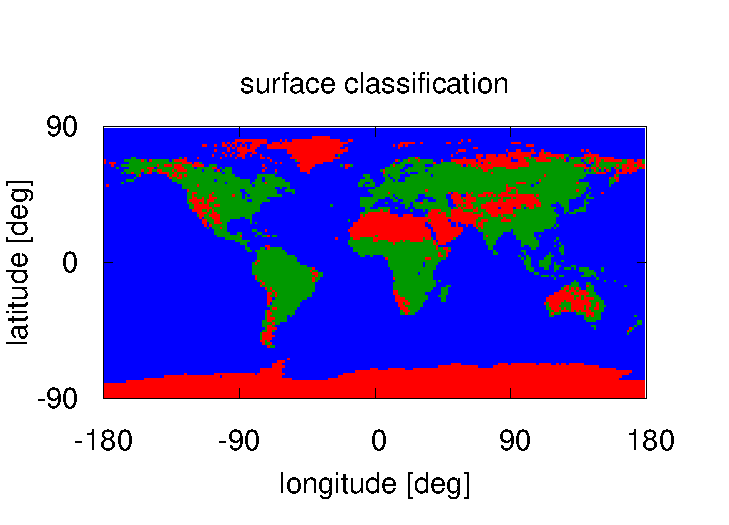
\includegraphics[width=\hsize]{IGBP_simplemap.pdf}
    \end{center}
     \end{minipage}
  \begin{minipage}{0.5\hsize}
    \begin{center}
    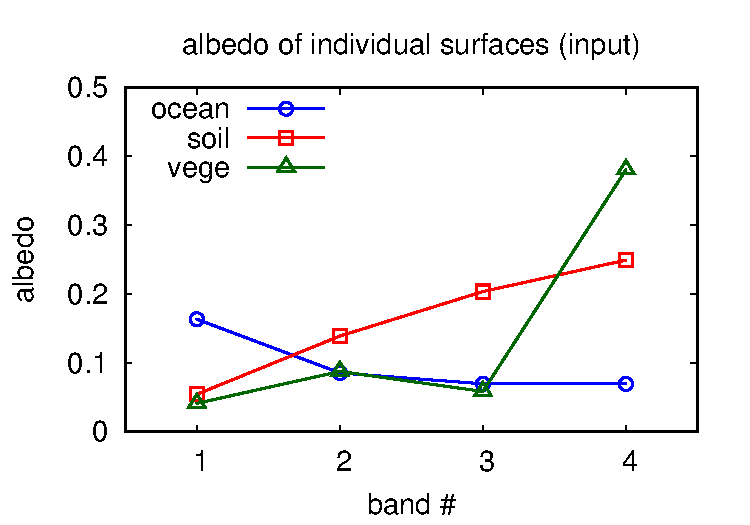
\includegraphics[width=\hsize]{mockdata_quadrature_bandsp.pdf}
    \end{center}
\end{minipage}
  \begin{minipage}{0.5\hsize}
    \begin{center}
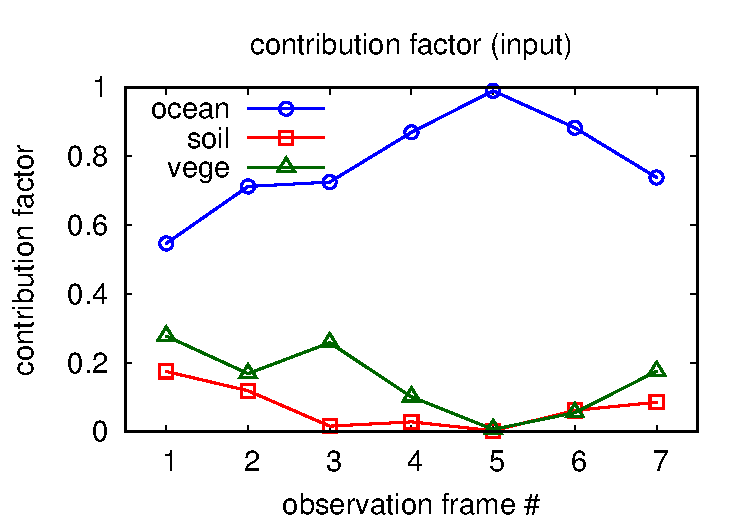
\includegraphics[width=\hsize]{mockdata_quadrature_factor.pdf}
    \end{center}
 \end{minipage}
   \begin{minipage}{0.5\hsize}
    \begin{center}
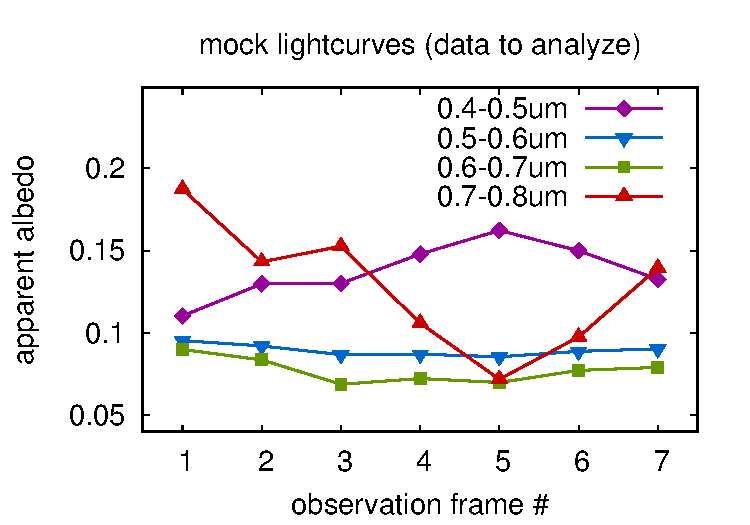
\includegraphics[width=\hsize]{mockdata_quadrature_lc.pdf}
    \end{center}
 \end{minipage}
    \caption{Our mock data based on Earth surface. }
\label{fig:mockdata}
\end{figure*}
%%%%%%%%%%%%%%%%%%%%%%%%%%%%%%%%%%%

Before applying to the observed data, we shall demonstrate the analysis procedure with a mock dataset with the known answer. 
For this purpose, we use a simplified albedo map of the Earth based on the IGBP classification. 
We re-classify the IGBP map into four surface types, ``ocean', ``vegetation', and ``soil'' and following Table 2 of \citet{Fujii2010} except that we merge ``snow'' into ``soil'' considering its small fraction. 
The upper left panel of Figure \ref{fig:mockdata} depicts such an surface classification. 
The reflectance spectra for these three surface types ($s_{kj}$) are adopted from ASTER spectral library \citep{Baldridge2009} in the same way as \citet{Fujii2010} (Figure 7 in that paper), and are shown in the upper right panel of Figure \ref{fig:mockdata}. 

We then compute the geometrically weighted area fraction of each surface type (``apparent covering fraction'' or $f^{\ast }_{ik}$) assuming an equatorial view at the quadrature, as is shown in the lower left panel of Figure \ref{fig:mockdata}. 
Specifically, we fix the sub-observer latitude at $0^{\circ }$, sub-observer at $0^{\circ }$, the sub-solar latitude at $0^{\circ }$, and sub-solar longitude at $90^{\circ }$. 
Using $s_{kj}$ and $f^{\ast }_{ik}$, we compute the apparent albedo at each observation frame, on the assumption that the surfaces are ``Lambert'' scatterers. The effect of atmosphere is completely ignored. 
The mock lightcurves created through the above-mentioned procedure is presented in the lower right panel of Figure \ref{fig:mockdata}. 

\newpage

%%%%%%%%%%%%%%%%%%%%%%%%%%%%%%%%%%%%%%%%%%%%%%%%%%%%%%%%%%%%%%
\subsection{PCA and Shrink-Wrapping}
\label{ss:shrinkwrap}
%%%%%%%%%%%%%%%%%%%%%%%%%%%%%%%%%%%%%%%%%%%%%%%%%%%%%%%%%%%%%%


Now, we analyze the mock data created in the preceding section (Figure \ref{fig:mockdata}). 
In this section, the result of PCA and shrink-wrapping are presented and discussed. 

PCA on the mock data indicated one dominant component (contribution: $\sim $98\%) and one minor component (contribution: $\sim $2\%). The residual is virtually zero, leaving 2 components in total, consistent with the assumption of 3 surface types. 
The corresponding principal components are shown in Figure \ref{fig:PCs}. 


%%%%%%%%%%%%%%%%%%%%%%%%%%%%%%%%%%%
\begin{figure}[th]
    \begin{center}
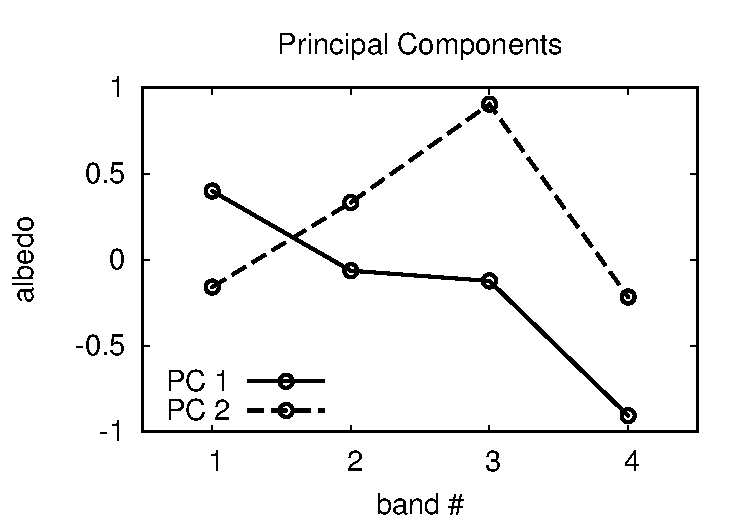
\includegraphics[width=0.9\hsize]{PCA_V_jn.pdf}
    \end{center}
    \caption{Principal Components. }
\label{fig:PCs}
\end{figure}
%%%%%%%%%%%%%%%%%%%%%%%%%%%%%%%%%%%


%%%%%%%%%%%%%%%%%%%%%%%%%%%%%%%%%%%
\begin{figure*}[bht]
    \begin{center}
%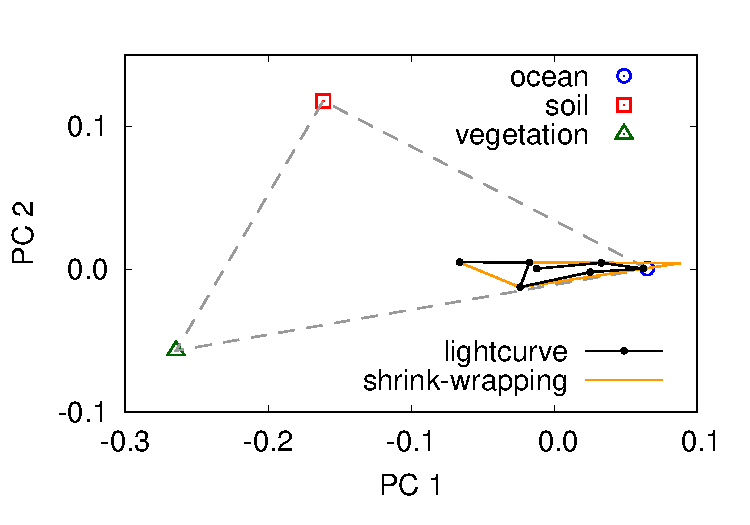
\includegraphics[width=\hsize]{PCA_projected.pdf}
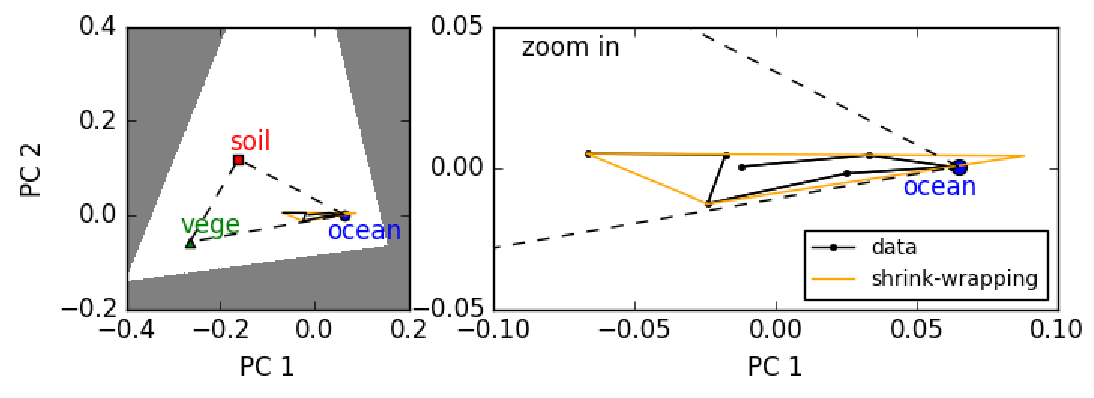
\includegraphics[width=\hsize]{mockdata_quadrature_PCplane.pdf}
    \end{center}
    \caption{Colors of 3 surface types and the light curves projected to the plane of 1st and 2nd principal components. }
\label{fig:shrinkwrap}
\end{figure*}
%%%%%%%%%%%%%%%%%%%%%%%%%%%%%%%%%%%

Then, we performed simplex shrink-wrapping analysis in the plane defined by these two principal components, based on the algorithm described in \citet{Fuhrmann1999}. 
The result are presented in Figure \ref{fig:shrinkwrap}. 
The black solid line indicates the trajectory of the light curves projected in this plane. 
The minimum-volume triangle that encloses the data points are found at the orange line in the same figure. 
For reference, the locations of the assumed three surface colors projected onto this plane are shown as points. 
As can be seen, the light curves the minimum-volume enclosure does not match the colors of physical surfaces, except for ocean. 
This is a natural consequence from the fact that the soil and vegetation are minor components and never dominate the surface in the illuminated and visible area, while the apparent covering fraction of ocean comes close to unity. 


\clearpage


%%%%%%%%%%%%%%%%%%%%%%%%%%%%%%%%%%%%%%%%%%%%%%%%%%%%%%%%%%%%%%
\subsection{[NEW] Effect of Regularization Term}
\label{ss:shrinkwrap}
%%%%%%%%%%%%%%%%%%%%%%%%%%%%%%%%%%%%%%%%%%%%%%%%%%%%%%%%%%%%%%

\subsubsection{Fitting with $\fast$}

%%%
\begin{eqnarray}
\mathcal{P}_{\fast} &=& \prod _k \left[ \frac{1}{(\sqrt{ 2 \pi })^{I} \sqrt{| \tilde \Sigma |} } \right. \\
&& \left. \times \exp \left\{ - \sum _{i,\,i'} (\fast ^{T})_{ki} \tilde \Sigma_{ii'} ^{-1} \fast_{i'k} \right\} \right] \\
\tilde \Sigma _{ii'} (\lambda,  \Delta_t ) &=& \exp \left( - \frac{|t_i- t_i'|^2}{2 \Delta_t^2} \right)
\end{eqnarray}
%%%

%%%
\begin{eqnarray}
- \log \mathcal{P}_{\fast} &\propto & \frac{1}{2} | \tilde \Sigma | + \mathcal{F}(\lambda, \Delta_t; \fast) \\
\mathcal{\tilde F}(\lambda, \Delta_t; \fast)&\equiv & \sum _k \sum_{i,\,i'} (\fast ^{T})_{ki} \tilde \Sigma_{ii'} ^{-1} \fast_{i'k}
\end{eqnarray}
%%%

...I think $\fast $ here should be zero mean for each $k$. 
%%%
\begin{equation}
\fast_{ik} \rightarrow ( \fast_{ik} - \fast^{(ave)}_k )
\end{equation}
%%%
In the following figures, the vertices of each triangle indicates the sample combination of the colors projected onto the principal component plane, and the colors is scaled by $\mathcal{\tilde F}^{\ast } (\Delta_t; \fast) = \lambda ^2 \mathcal{\tilde F}$. 


\subsubsection{Concerns}

%%%
\begin{itemize}
\item $\fast_{lk}$'s or $f_{lk}$'s are not mutually independent. (Sum is unity.) 
\item Same regularization 
\end{itemize}
%%%



%%%%%%%%%%%%%%%%%%%%%%%%%%%%%%%%%%%
\begin{figure*}[b]
    \begin{minipage}{0.33\hsize}
    \begin{center}
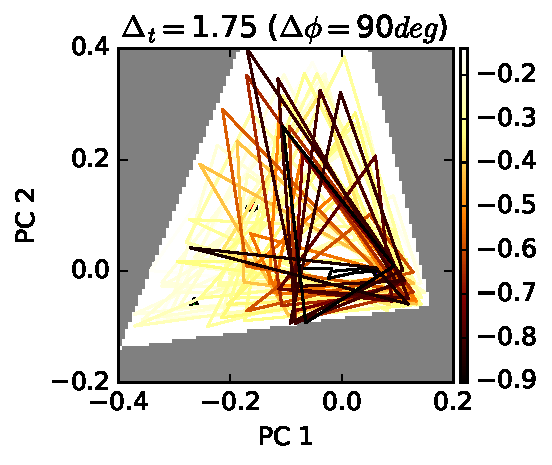
\includegraphics[width=\hsize]{mockdata_90deg_time7_lc_regf_PCplane_l90deg_2013.pdf}
    \end{center}
    \end{minipage}
    \begin{minipage}{0.33\hsize}
    \begin{center}
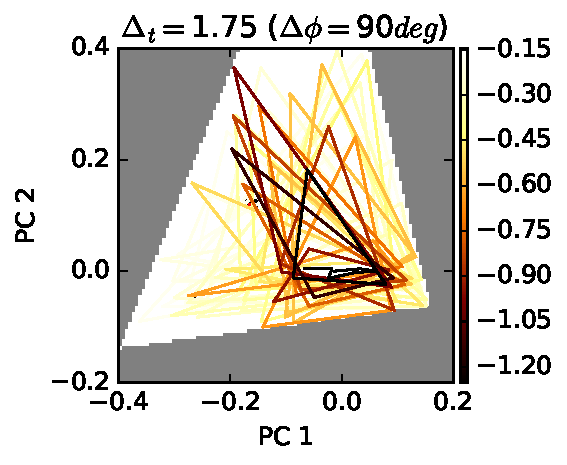
\includegraphics[width=\hsize]{mockdata_90deg_time7_lc_regf_PCplane_l90deg_2017.pdf}
    \end{center}
    \end{minipage}
    \begin{minipage}{0.33\hsize}
    \begin{center}
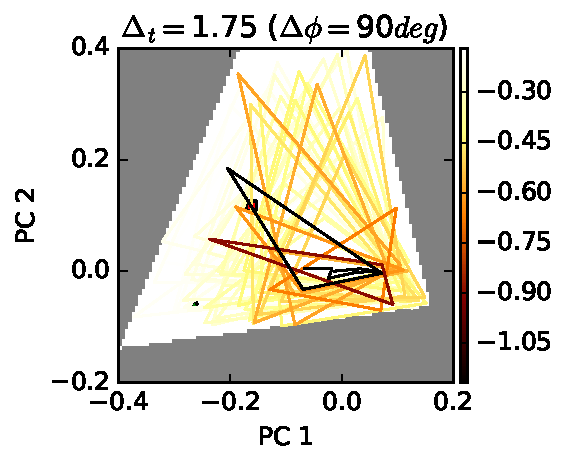
\includegraphics[width=\hsize]{mockdata_90deg_time7_lc_regf_PCplane_l90deg_2019.pdf}
    \end{center}
    \end{minipage}    
    \caption{The vertices of each triangle indicates the sample combination of the colors projected onto the principal component plane, and the colors is scaled by $\mathcal{\tilde F}^{\ast }$ with $\Delta_t=1.75$ \color{red} when the lightcurves are sampled 11 times in one rotation. \color{black}.The difference between the three panels is just the seed for \url{np.randam.uniform}}
\label{fig:regterm}
\end{figure*}
%%%%%%%%%%%%%%%%%%%%%%%%%%%%%%%%%%%


%%%%%%%%%%%%%%%%%%%%%%%%%%%%%%%%%%%
\begin{figure*}[b]
    \begin{minipage}{0.33\hsize}
    \begin{center}
\includegraphics[width=\hsize]{mockdata_90deg_time7_lc_regf_PCplane_l120deg_2013.pdf}
    \end{center}
    \end{minipage}
    \begin{minipage}{0.33\hsize}
    \begin{center}
\includegraphics[width=\hsize]{mockdata_90deg_time7_lc_regf_PCplane_l120deg_2017.pdf}
    \end{center}
    \end{minipage}
    \begin{minipage}{0.33\hsize}
    \begin{center}
\includegraphics[width=\hsize]{mockdata_90deg_time7_lc_regf_PCplane_l120deg_2019.pdf}
    \end{center}
    \end{minipage}
    \caption{The vertices of each triangle indicates the sample combination of the colors projected onto the principal component plane, and the colors is scaled by $\mathcal{\tilde F}^{\ast }$ with $\Delta_t\sim 2.3$ \color{red} when the lightcurves are sampled 11 times in one rotation. \color{black}. The difference between the three panels is just the seed for \url{np.randam.uniform}}
\label{fig:regterm}
\end{figure*}
%%%%%%%%%%%%%%%%%%%%%%%%%%%%%%%%%%%

%%%%%%%%%%%%%%%%%%%%%%%%%%%%%%%%%%%
\begin{figure*}[b]
    \begin{minipage}{0.33\hsize}
    \begin{center}
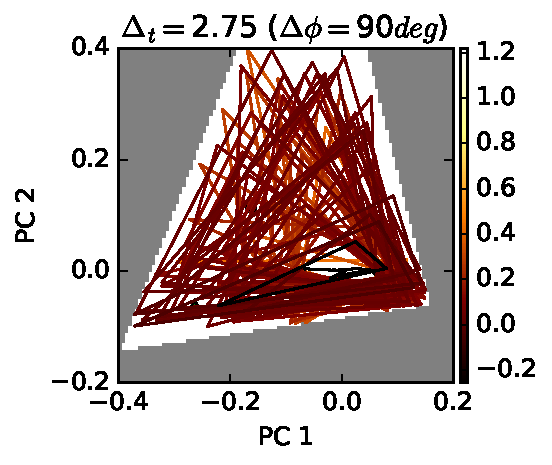
\includegraphics[width=\hsize]{mockdata_90deg_time11_lc_regf_PCplane_l90deg_2013.pdf}
    \end{center}
    \end{minipage}
    \begin{minipage}{0.33\hsize}
    \begin{center}
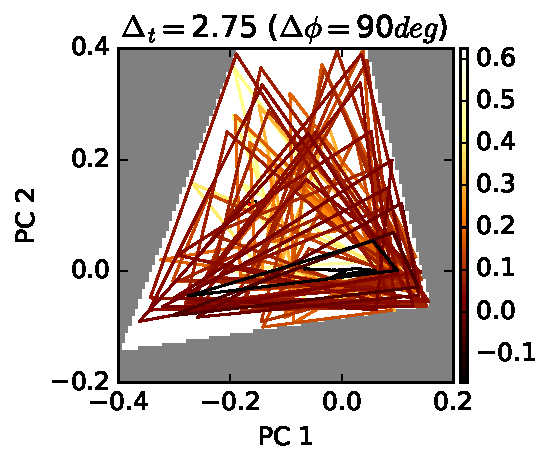
\includegraphics[width=\hsize]{mockdata_90deg_time11_lc_regf_PCplane_l90deg_2017.pdf}
    \end{center}
    \end{minipage}
    \begin{minipage}{0.33\hsize}
    \begin{center}
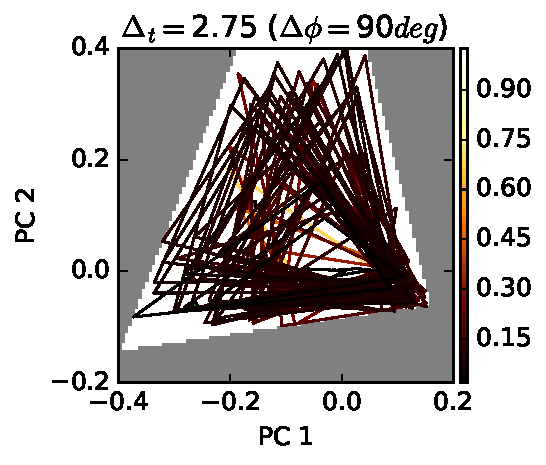
\includegraphics[width=\hsize]{mockdata_90deg_time11_lc_regf_PCplane_l90deg_2019.pdf}
    \end{center}
    \end{minipage}
    \caption{The vertices of each triangle indicates the sample combination of the colors projected onto the principal component plane, and the colors is scaled by $\mathcal{\tilde F}^{\ast }$ \color{red} when the lightcurves are sampled 11 times in one rotation. \color{black} The difference between the three panels is just the seed for \url{np.randam.uniform}}
\label{fig:regterm}
\end{figure*}
%%%%%%%%%%%%%%%%%%%%%%%%%%%%%%%%%%%


%%%%%%%%%%%%%%%%%%%%%%%%%%%%%%%%%%%
\begin{figure*}[b]
    \begin{minipage}{0.33\hsize}
    \begin{center}
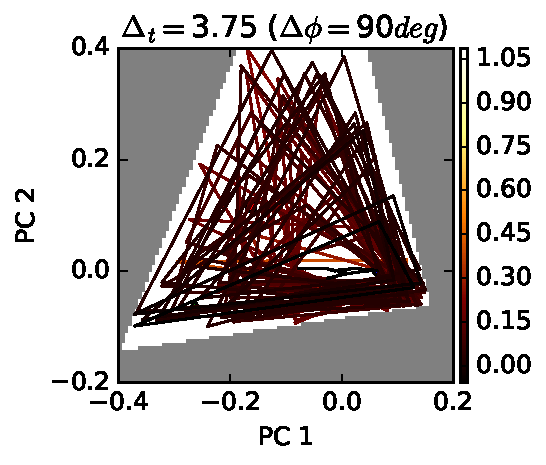
\includegraphics[width=\hsize]{mockdata_90deg_time15_lc_regf_PCplane_l90deg_2013.pdf}
    \end{center}
    \end{minipage}
    \begin{minipage}{0.33\hsize}
    \begin{center}
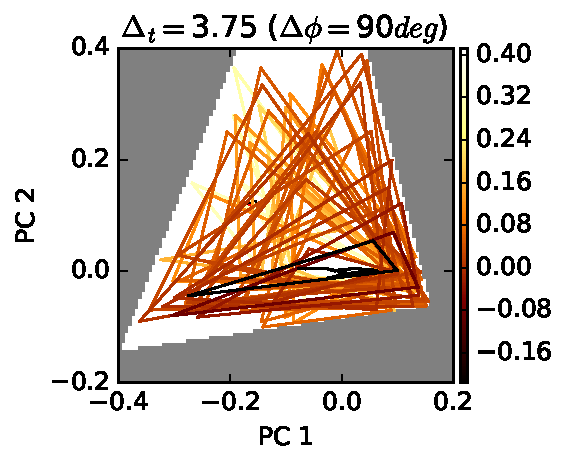
\includegraphics[width=\hsize]{mockdata_90deg_time15_lc_regf_PCplane_l90deg_2017.pdf}
    \end{center}
    \end{minipage}
    \begin{minipage}{0.33\hsize}
    \begin{center}
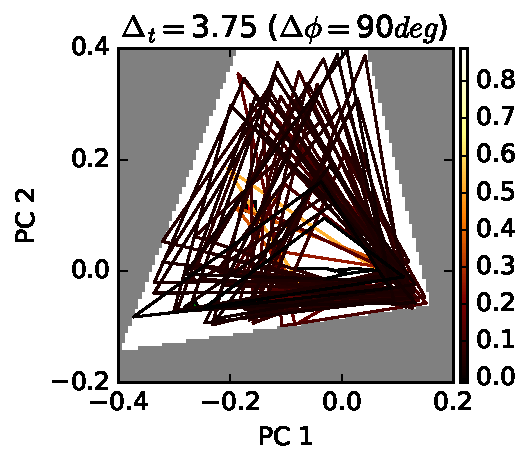
\includegraphics[width=\hsize]{mockdata_90deg_time15_lc_regf_PCplane_l90deg_2019.pdf}
    \end{center}
    \end{minipage}
    \caption{The vertices of each triangle indicates the sample combination of the colors projected onto the principal component plane, and the colors is scaled by $\mathcal{\tilde F}^{\ast }$ \color{red} when the lightcurves are sampled 15 times in one rotation. \color{black}. The difference between the three panels is just the seed for \url{np.randam.uniform}}
\label{fig:regterm}
\end{figure*}
%%%%%%%%%%%%%%%%%%%%%%%%%%%%%%%%%%%


%%%%%%%%%%%%%%%%%%%%%%%%%%%%%%%%%%%
\begin{figure*}[b]
    \begin{minipage}{0.33\hsize}
    \begin{center}
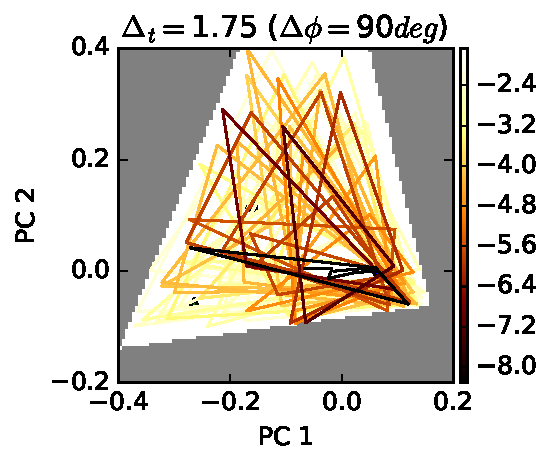
\includegraphics[width=\hsize]{mockdata_90deg_time7_lc_2_regf_PCplane_l90deg_2013.pdf}
    \end{center}
    \end{minipage}
    \begin{minipage}{0.33\hsize}
    \begin{center}
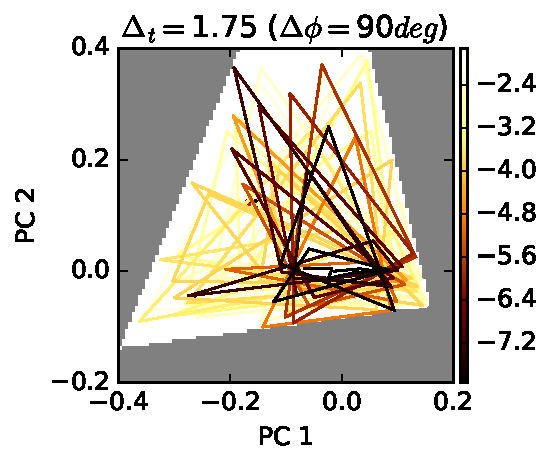
\includegraphics[width=\hsize]{mockdata_90deg_time7_lc_2_regf_PCplane_l90deg_2017.pdf}
    \end{center}
    \end{minipage}
    \begin{minipage}{0.33\hsize}
    \begin{center}
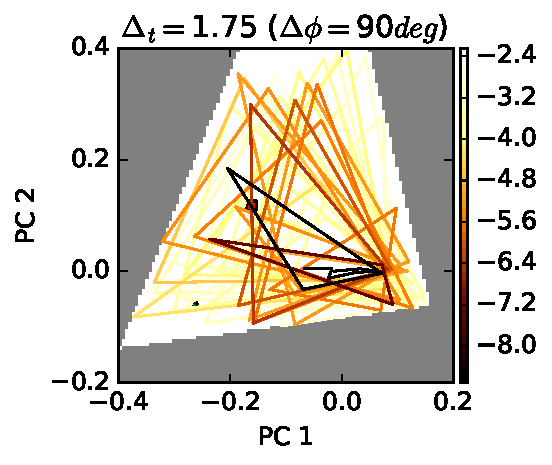
\includegraphics[width=\hsize]{mockdata_90deg_time7_lc_2_regf_PCplane_l90deg_2019.pdf}
    \end{center}
    \end{minipage}    
    \caption{The vertices of each triangle indicates the sample combination of the colors projected onto the principal component plane, and the colors is scaled by $\mathcal{\tilde F}^{\ast }$ with $\Delta_t=1.75$ \color{red} when the lightcurves are sampled 7 times in one rotation. \color{black}.The difference between the three panels is just the seed for \url{np.randam.uniform}. In the regularization term, not $f_{lk}$ but $(f_{lk}-f_{k}^{\rm (ave)})/f_{k}^{\rm (ave)}$ are used where $f_{k}^{\rm (ave)} = (\sum_l f_{lk})/L$. }
\label{fig:regterm}
\end{figure*}
%%%%%%%%%%%%%%%%%%%%%%%%%%%%%%%%%%%


%%%%%%%%%%%%%%%%%%%%%%%%%%%%%%%%%%%
\begin{figure*}[b]
    \begin{minipage}{0.33\hsize}
    \begin{center}
\includegraphics[width=\hsize]{mockdata_90deg_time7_lc_g_regf_PCplane_l90deg_2013.pdf}
    \end{center}
    \end{minipage}
    \begin{minipage}{0.33\hsize}
    \begin{center}
\includegraphics[width=\hsize]{mockdata_90deg_time7_lc_g_regf_PCplane_l90deg_2017.pdf}
    \end{center}
    \end{minipage}
    \begin{minipage}{0.33\hsize}
    \begin{center}
\includegraphics[width=\hsize]{mockdata_90deg_time7_lc_g_regf_PCplane_l90deg_2019.pdf}
    \end{center}
    \end{minipage}    
    \caption{The vertices of each triangle indicates the sample combination of the colors projected onto the principal component plane, and the colors is scaled by $\mathcal{\tilde F}^{\ast }$ with $\Delta_t=1.75$ \color{red} when the lightcurves are sampled 7 times in one rotation. \color{black}.The difference between the three panels is just the seed for \url{np.randam.uniform}. In the regularization term, not $f_{lk}$ but $g_{lk}$ are used. }
\label{fig:regterm}
\end{figure*}
%%%%%%%%%%%%%%%%%%%%%%%%%%%%%%%%%%%


%%%%%%%%%%%%%%%%%%%%%%%%%%%%%%%%%%%
\begin{figure*}[b]
    \begin{minipage}{0.5\hsize}
    \begin{center}
\includegraphics[width=\hsize]{simpleIGBP_quadrature_lc_l90deg_2013_X_albd_jk_best.pdf}
    \end{center}
    \end{minipage}
    \begin{minipage}{0.5\hsize}
    \begin{center}
\includegraphics[width=\hsize]{simpleIGBP_quadrature_lc_l90deg_2013_X_area_ik_best.pdf}
    \end{center}
    \end{minipage}
    \caption{Solution with smallest regularization term when $\Delta_t=1.75$ ($\Delta \phi = 90^{\circ }$).}
\label{fig:regterm}
\end{figure*}
%%%%%%%%%%%%%%%%%%%%%%%%%%%%%%%%%%%

%%%%%%%%%%%%%%%%%%%%%%%%%%%%%%%%%%%
%\begin{figure*}[b]
%    \begin{minipage}{0.5\hsize}
%    \begin{center}
%\includegraphics[width=\hsize]{simpleIGBP_quadrature_lc_l120deg_2013_X_albd_jk_best.pdf}
%    \end{center}
%    \end{minipage}
%    \begin{minipage}{0.5\hsize}
%    \begin{center}
%\includegraphics[width=\hsize]{simpleIGBP_quadrature_lc_l120deg_2013_X_area_ik_best.pdf}
%    \end{center}
%    \end{minipage}
%    \caption{Solution with smallest regularization term. }
%\label{fig:regterm}
%\end{figure*}
%%%%%%%%%%%%%%%%%%%%%%%%%%%%%%%%%%%




\clearpage

\subsubsection{Fitting with $f$}

What if $f$ is used instead of $\fast$ in fitting?

From equation (\ref{eq:d_f_s}), the solution for $f_{lk} s_{kj}$ that is found through the least-square method is
%%%
\begin{equation}
\sum_i (W^{+})_{li} d_{ij} = \sum_k f_{lk} s_{kj}
\end{equation}
%%%
So, with an analogy to equation (\ref{eq:d_f_ast_s}), we could make similar plots of the principal components plane (with the principal components found from $\sum_i (W^{+})_{li} d_{ij}$ instead of $d_{ij}$). 

Then, the regularization term would be $\mathcal{F}^{\ast } (\Delta_{\phi }; f) = \lambda ^2 \mathcal{F}$ will be used where
%%%
\begin{equation}
\mathcal{F}(\lambda, \Delta_{\phi }; f)\equiv  \sum _k \sum_{i,\,i'} (f^{T})_{ki} \Sigma_{ii'} ^{-1} f_{i'k}. 
\end{equation}
%%%


%%%%%%%%%%%%%%%%%%%%%%%%%%%%%%%%%%%
\begin{figure*}[h]
    \begin{minipage}{0.33\hsize}
    \begin{center}
\includegraphics[width=\hsize]{simpleIGBP_quadrature_lc_fitmap_regf_PCplane_l90deg_2013.pdf}
    \end{center}
    \end{minipage}
    \begin{minipage}{0.33\hsize}
    \begin{center}
\includegraphics[width=\hsize]{simpleIGBP_quadrature_lc_fitmap_regf_PCplane_l90deg_2017.pdf}
    \end{center}
    \end{minipage}
    \begin{minipage}{0.33\hsize}
    \begin{center}
\includegraphics[width=\hsize]{simpleIGBP_quadrature_lc_fitmap_regf_PCplane_l90deg_2019.pdf}
    \end{center}
    \end{minipage}
    \caption{The vertices of each triangle indicates the sample combination of the colors projected onto the principal component plane, and the colors is scaled by $\mathcal{F}^{\ast }$ with $\Delta_t\sim 1.25$. The difference between the three panels is just the seed for \url{np.randam.uniform}.}
\label{fig:regterm}
\end{figure*}
%%%%%%%%%%%%%%%%%%%%%%%%%%%%%%%%%%%


%%%%%%%%%%%%%%%%%%%%%%%%%%%%%%%%%%%
\begin{figure*}[h]
    \begin{minipage}{0.5\hsize}
    \begin{center}
\includegraphics[width=\hsize]{simpleIGBP_quadrature_lc_fitmap_l90deg_2013_X_albd_jk_best.pdf}
    \end{center}
    \end{minipage}
    \begin{minipage}{0.5\hsize}
    \begin{center}
\includegraphics[width=\hsize]{simpleIGBP_quadrature_lc_fitmap_l90deg_2013_X_area_ik_best.pdf}
    \end{center}
    \end{minipage}
    \caption{Solution with smallest regularization term when $\Delta \phi = 90^{\circ }$. }
\label{fig:regterm}
\end{figure*}
%%%%%%%%%%%%%%%%%%%%%%%%%%%%%%%%%%%

\bibliography{ref}

\acknowledgments

ISSI Exo-cartography workshop in Bern. 

\end{document}

\clearpage

%%%%%%%%%%%%%%%%%%%%%%%%%%%%%%%%%%%
\begin{figure*}[!htbp]
    \begin{center}
%\includegraphics[width=\hsize]{xmed_std_regtime_s1e-2.pdf}
%\includegraphics[width=\hsize]{xmed_std_regtime_s1e-4.pdf}
\includegraphics[width=\hsize]{xmed_std_regtime_l1e-2.pdf}
\includegraphics[width=\hsize]{xmed_std_regtime_l1e-4.pdf}
    \end{center}
    \caption{Regularization in terms of time. Upper: $\lambda = 0.01$. Lower: $\lambda = 0.0001$. \memoYF{But the MC chains do not converge after 5000 steps!}}
\label{fig:shrinkwrap}
\end{figure*}
%%%%%%%%%%%%%%%%%%%%%%%%%%%%%%%%%%%







%%%%%%%%%%%%%%%%%%%%%%%%%%%%%%%%%%%
\begin{figure*}[!htbp]
    \begin{center}
\includegraphics[width=\hsize]{xmed_std_reglong_l1e-2.pdf}
%\includegraphics[width=\hsize]{xmed_std_reglong_l1e-4.pdf}
    \end{center}
    \caption{Regularization in terms of longitude. Upper: $\sigma = 0.01$. Lower: $\sigma = 0.0001$. \memoYF{But the MC chains do not converge after 5000 steps!}}
\label{fig:xmed_std_reglong_l1e-2}
\end{figure*}
%%%%%%%%%%%%%%%%%%%%%%%%%%%%%%%%%%%

%%%%%%%%%%%%%%%%%%%%%%%%%%%%%%%%%%%
\begin{figure*}[!htbp]
    \begin{center}
\includegraphics[width=\hsize]{reglong_l1e-2_trace0.png}
\includegraphics[width=\hsize]{reglong_l1e-2_trace8.png}
\includegraphics[width=\hsize]{reglong_l1e-2_trace13.png}
    \end{center}
    \caption{Examples of MC chains in estimating $\{ f,\,s\}$ with $\lambda = 0.01$, corresponding to Figure \ref{fig:xmed_std_reglong_l1e-2}. }
\label{fig:shrinkwrap}
\end{figure*}
%%%%%%%%%%%%%%%%%%%%%%%%%%%%%%%%%%%


%%%%%%%%%%%%%%%%%%%%%%%%%%%%%%%%%%%
%\begin{figure*}[!htbp]
%    \begin{center}
%\includegraphics[width=\hsize]{xmed_std_reglong_s1e-4.pdf}
%    \end{center}
%    \caption{Result of estimation for $\{ f,\,s\}$ with $\lambda = 0.0001$. \memoYF{MC chains do not fully converge in 5000 steps.}}
%\label{fig:shrinkwrap}
%\end{figure*}
%%%%%%%%%%%%%%%%%%%%%%%%%%%%%%%%%%%


%%%%%%%%%%%%%%%%%%%%%%%%%%%%%%%%%%%
%\begin{figure*}[!htbp]
%    \begin{center}
%\includegraphics[width=\hsize]{xmed_std_time.pdf}
%\includegraphics[width=\hsize]{xmed_std_longitude.pdf}
%    \end{center}
%    \caption{Left: result of estimation for $\{ \fast,\,s\}$. Right: result of estimation for $\{ f,\,s\}$}
%\label{fig:shrinkwrap}
%\end{figure*}
%%%%%%%%%%%%%%%%%%%%%%%%%%%%%%%%%%%




\clearpage

\acknowledgments

\bibliography{ref}

\newpage

\appendix

%%%%%%%%%%%%%%%%%%%%%%%%%%%%%%%%%%%%%%%%%%%%%%%%%%%%%%%%%%%%%%%%%%%
\section{Discussion}
\label{s:discussion}
%%%%%%%%%%%%%%%%%%%%%%%%%%%%%%%%%%%%%%%%%%%%%%%%%%%%%%%%%%%%%%%%%%%


%%%%%%%%%%%%%%%%%%%%%%%%%%%%%%%%%%%%%%%%%%%%%%%%%%%%%%%%%%%%%%
\subsection{Uncertainty in Radius}
\label{ss:radius}
%%%%%%%%%%%%%%%%%%%%%%%%%%%%%%%%%%%%%%%%%%%%%%%%%%%%%%%%%%%%%%


%%%%%%%%%%%%%%%%%%%%%%%%%%%%%%%%%%%%%%%%%%%%%%%%%%%%%%%%%%%%%%%%%%%
\section{Summary}
\label{s:summary}
%%%%%%%%%%%%%%%%%%%%%%%%%%%%%%%%%%%%%%%%%%%%%%%%%%%%%%%%%%%%%%%%%%%




\acknowledgments

\bibliography{ref}

\appendix


%%%%%%%%%%%%%%%%%%%%%%%%%%%%%%%%%%%%%%%%%%%%%%%%%%%%%%%%%%%%%%%%%%%
\section{Application to 4 EPOXI observations of the Earth}
\label{s:epoxi}
%%%%%%%%%%%%%%%%%%%%%%%%%%%%%%%%%%%%%%%%%%%%%%%%%%%%%%%%%%%%%%%%%%%

%%%%%%%%%%%%%%%%%%%%%%%%%%%%%%%%%%%%%%%%%%%%%%%%%%%%%%%%%%%%%%
\subsection{EPOXI data}
\label{ss:epoxidata}
%%%%%%%%%%%%%%%%%%%%%%%%%%%%%%%%%%%%%%%%%%%%%%%%%%%%%%%%%%%%%%

%%%%%%%%%%%%%%%%%%%%%%%%%%%%%%%%%%%
\begin{figure*}[b!]
    \begin{center}
\includegraphics[width=\hsize]{EPOXI_vislightcurve_4obs.pdf}
    \end{center}
    \caption{4 light curves of the Earth obtained with EPOXI mission.}
\label{fig:EPOXIlc}
\end{figure*}
%%%%%%%%%%%%%%%%%%%%%%%%%%%%%%%%%%%

We now apply our framework to the observed multi-band reflected light curves of the Earth obtained with EPOXI \citep{Livengood2011, Cowan2011}. 
There are 7 photometric filters from about 300 nm to 1000 nm, each of which has roughly 100-nm band width. 
In total, 5 series of observations were conducted, each of which spans $\sim $24 hours with 1-hour intervals. 
Since one of them includes lunar transit in front of the Earth and the interpretation is not straightforward, we just remove it from our data and consider only 4 series of observations, which were conducted on March 2008, June 2008, March 2009, and October 2009. 
The data are presented in Figure \ref{fig:EPOXIlc} in terms of {\it apparent albedo}. 

The geometrical configuration among the star, the target (the Earth), and the detector varies from observation to observation. 
The information is summarized in \citet{Cowan2011}, but we also outline in Table \ref{tab:EPOXI} just for reference. 

%%%%%%%%%%%%%%%%%%%%%%%%%%%%%%%%%%%
\begin{figure*}[!bt]
    \begin{center}
    \includegraphics[width=\hsize]{June_xmed_std_GPReg.pdf}
    \end{center}
    \caption{Result of inversion of EPOXI June data. \memoYF{to be revised}}
\label{fig:mcmc_June_tmp}
\end{figure*}
%%%%%%%%%%%%%%%%%%%%%%%%%%%%%%%%%%%

%%%%%%%%%%%%%%%%%%%%%%%%%%%%%%%%%%%
\begin{table*}[htp]
\caption{EPOXI Observations}
\begin{center}
\begin{tabular}{lcccc} \hline \hline
& Equator (equinox) & Equator (solstice) & North & South \\ \hline
Date & 2008 Mar 18-19 & 2008 Jun 4-5 & 2009 Mar 27-28 & 2009 Oct 4-5 \\ 
Phase & $57.7^{\circ }$ & $76.6^{\circ }$ & $85.9^{\circ }$ & $86.4^{\circ }$ \\ 
average sub-solar latitude & $-0.4^{\circ }$ & $22.6^{\circ }$ & $3.0^{\circ }$ & $-4.6^{\circ }$ \\
average sub-observer latitude & $1.6^{\circ }$ & $0.3^{\circ }$ & $61.5^{\circ }$ & $-73.7^{\circ }$  \\
initial sub-solar longitude & $267.6^{\circ }$ & $286.0^{\circ }$ & $296.7^{\circ }$ & $33.2^{\circ }$ \\
initial sub-observer longitude & $210.1^{\circ }$ & $210.5^{\circ }$ & $210.1^{\circ }$ & $300.6^{\circ }$ \\ \hline
\end{tabular}
\end{center}
\label{tab:EPOXI}
\end{table*}%
%%%%%%%%%%%%%%%%%%%%%%%%%%%%%%%%%%%


\end{document}
